\begin{table}[!p]
\vspace*{-\baselineskip}
\hspace*{-5mm}
%\begin{tabular}{r@{}c@{\,}c@{\,}c@{\,}c@{\,}c@{}c@{}c}
%\begin{tabular}{r@{}p{2.05cm}@{\,}p{2.05cm}@{\,}p{2.05cm}@{\,}p{2.05cm}@{\,}p{2.05cm}@{}p{2.05cm}@{}p{2.05cm}}
\begin{tabular}{r@{}p{2.0cm}@{}p{2.0cm}@{}p{2.0cm}@{}p{2.0cm}@{}p{2.0cm}@{}p{2.0cm}@{}p{2.0cm}}
 & \textbf{~~~~~250} & \textbf{~~~~~500} & \textbf{~~~~1000} & \textbf{~~~~2000} & \textbf{~~~~5000} & \textbf{~~~10000} & \textbf{~~~15000} \\
\textsc{mwst~} &
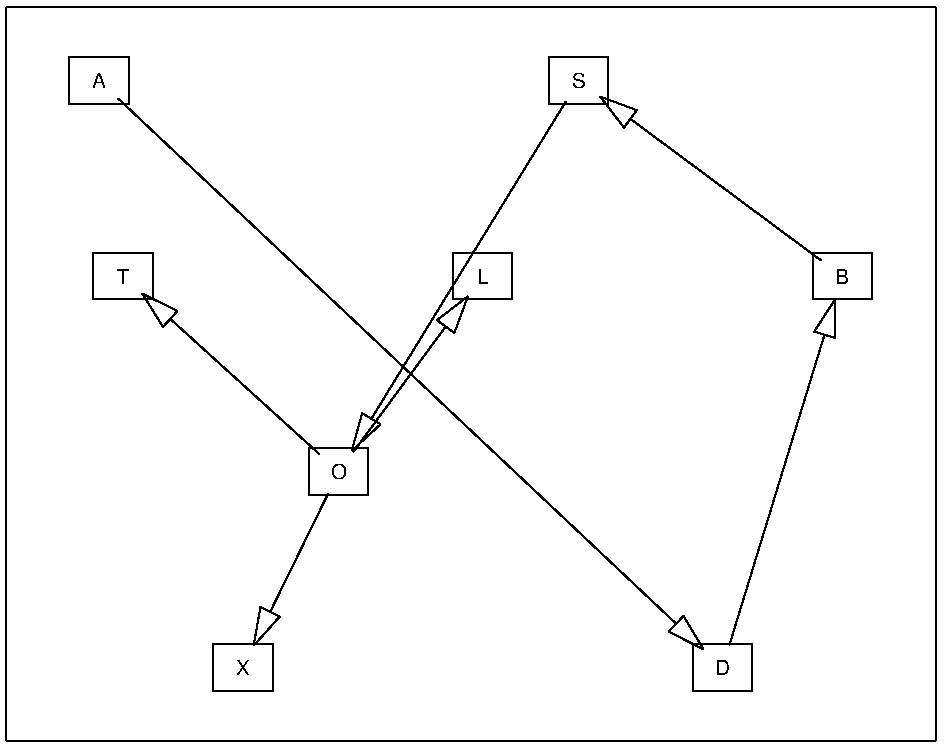
\includegraphics[width=20.3mm, height=14.25mm]{fig/11-Sep-2003-14-42-00-dag-asia250-MSWT-RES} &
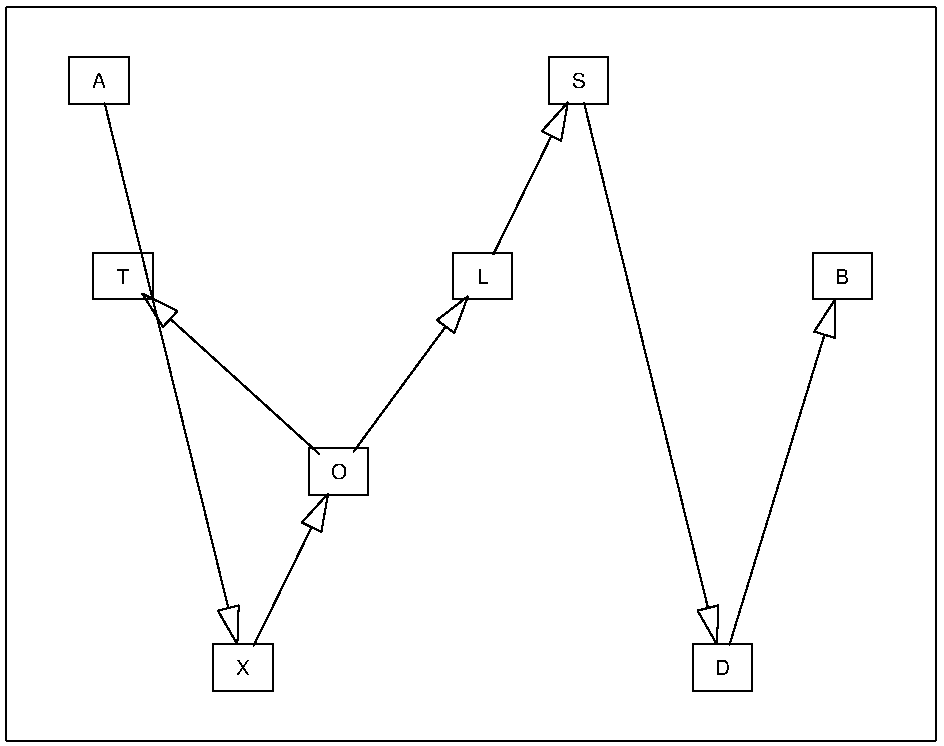
\includegraphics[width=20.3mm, height=14.25mm]{fig/11-Aug-2003-13-48-14-dag-asia500-MSWT-RES} &
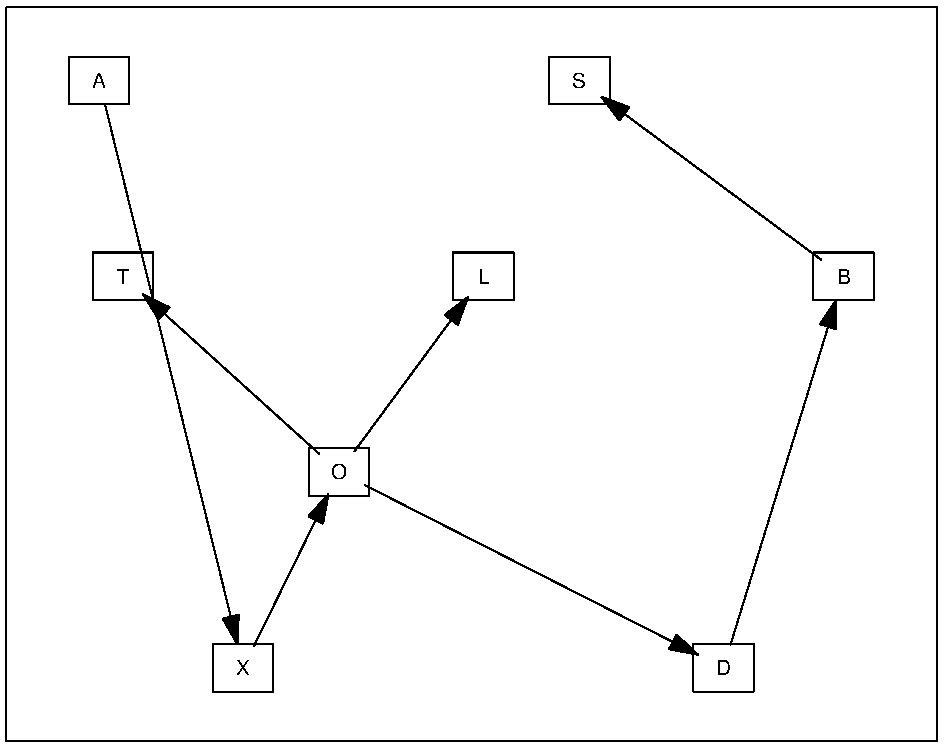
\includegraphics[width=20.3mm, height=14.25mm]{fig/19-Feb-2003-16-04-58-dag-asia1000-MSWT-RES} &
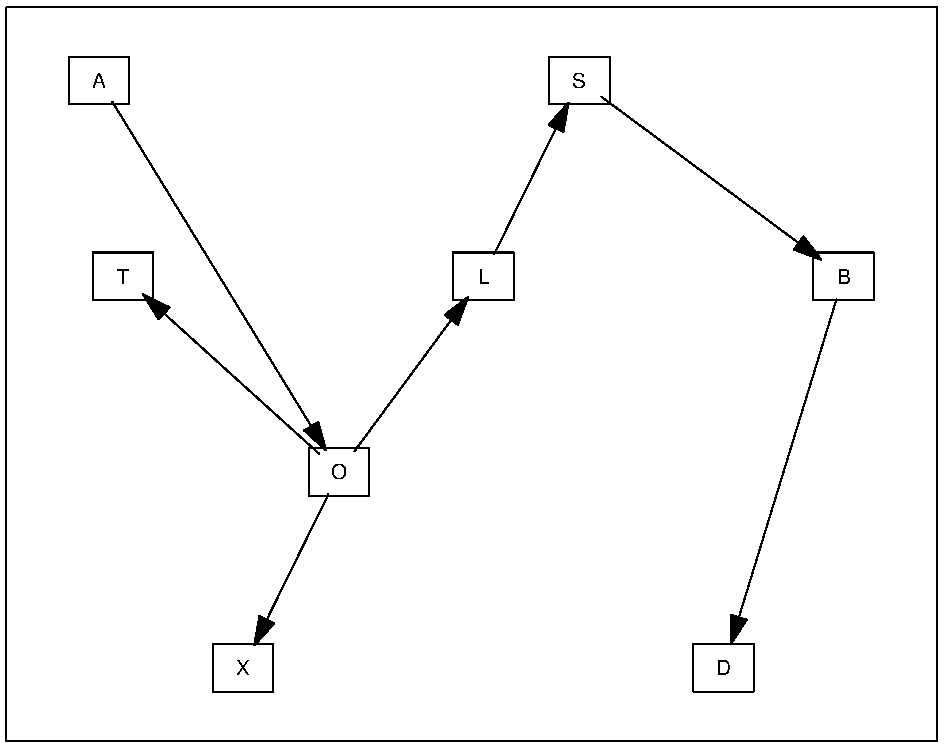
\includegraphics[width=20.3mm, height=14.25mm]{fig/19-Feb-2003-16-04-58-dag-asia2000-MSWT-RES} &
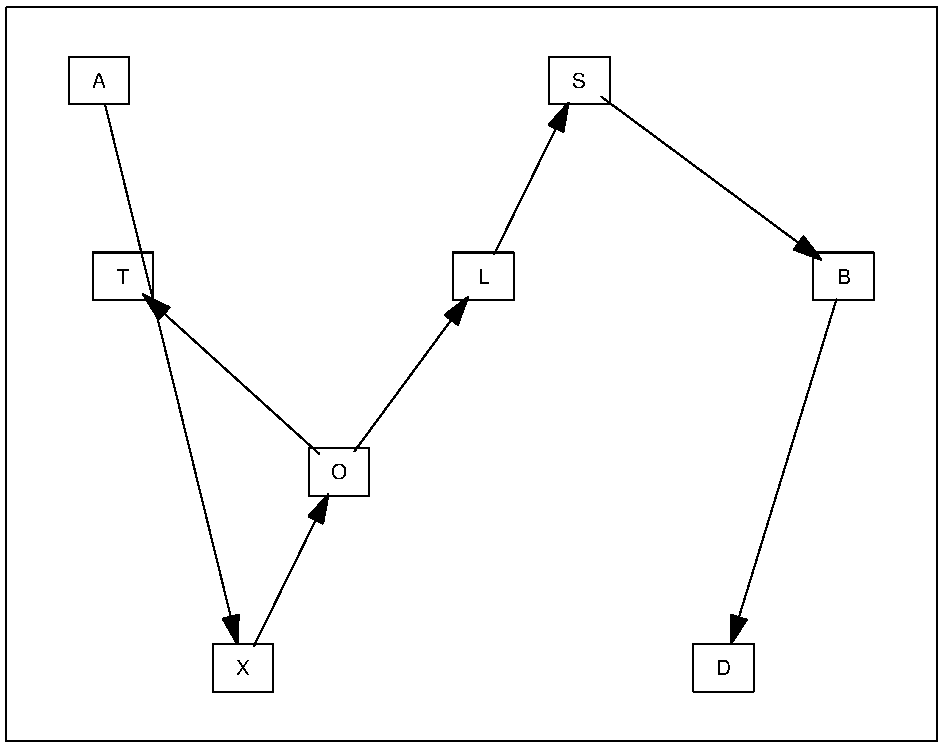
\includegraphics[width=20.3mm, height=14.25mm]{fig/19-Feb-2003-16-04-58-dag-asia5000-MSWT-RES} &
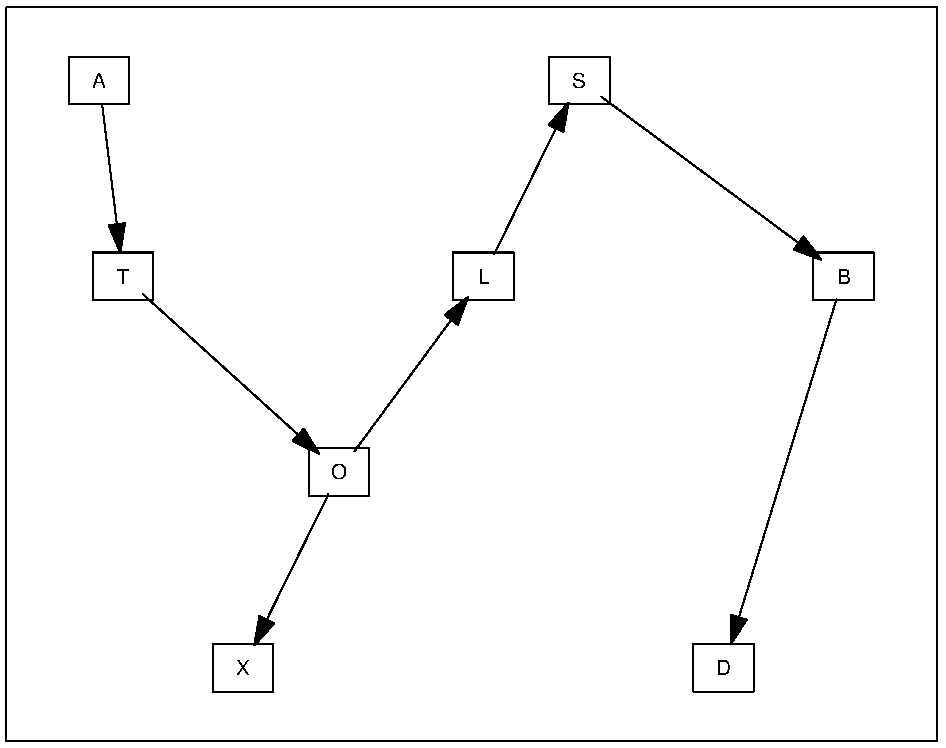
\includegraphics[width=20.3mm, height=14.25mm]{fig/19-Feb-2003-16-04-58-dag-asia10000-MSWT-RES} &
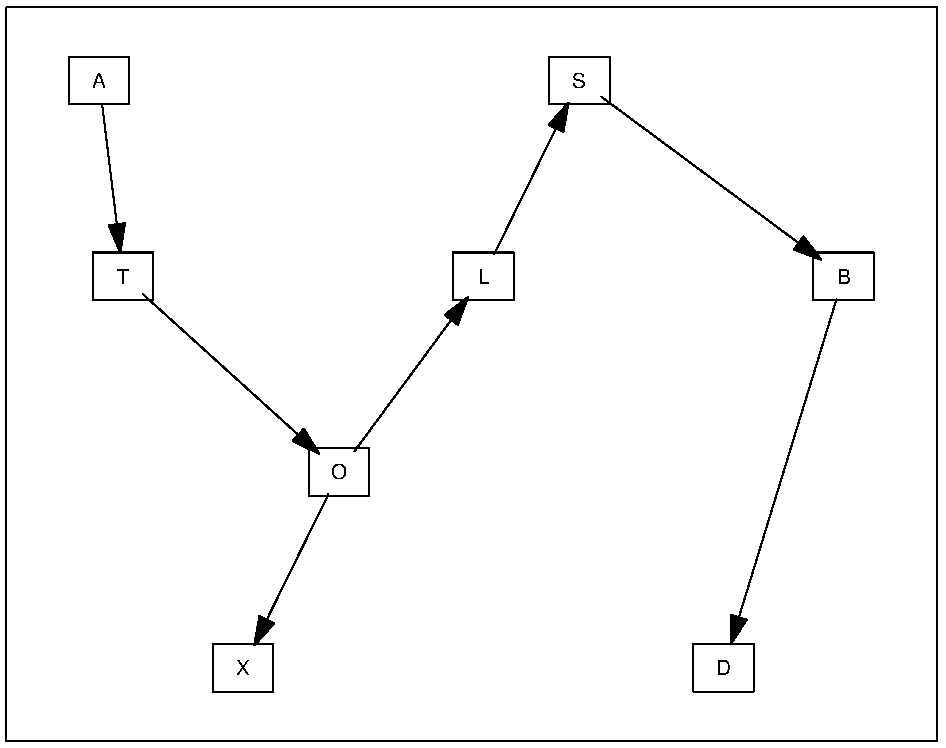
\includegraphics[width=20.3mm, height=14.25mm]{fig/19-Feb-2003-16-04-58-dag-asia15000-MSWT-RES} \\
& 9;-68837 & 10;-69235 & 8;-68772 & 6;-68704 & 7;-68704 & 3;-68694 & 3; -68694 \\
\textsc{pc~} &
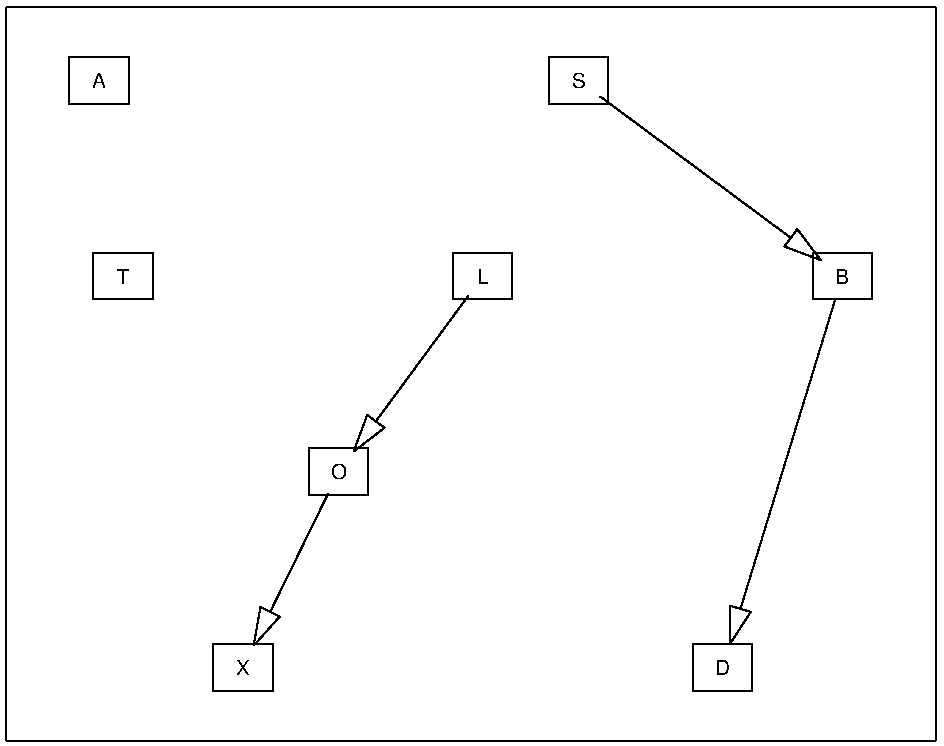
\includegraphics[width=20.3mm, height=14.25mm]{fig/11-Sep-2003-14-27-53-dag-asia250-PC-RES} &
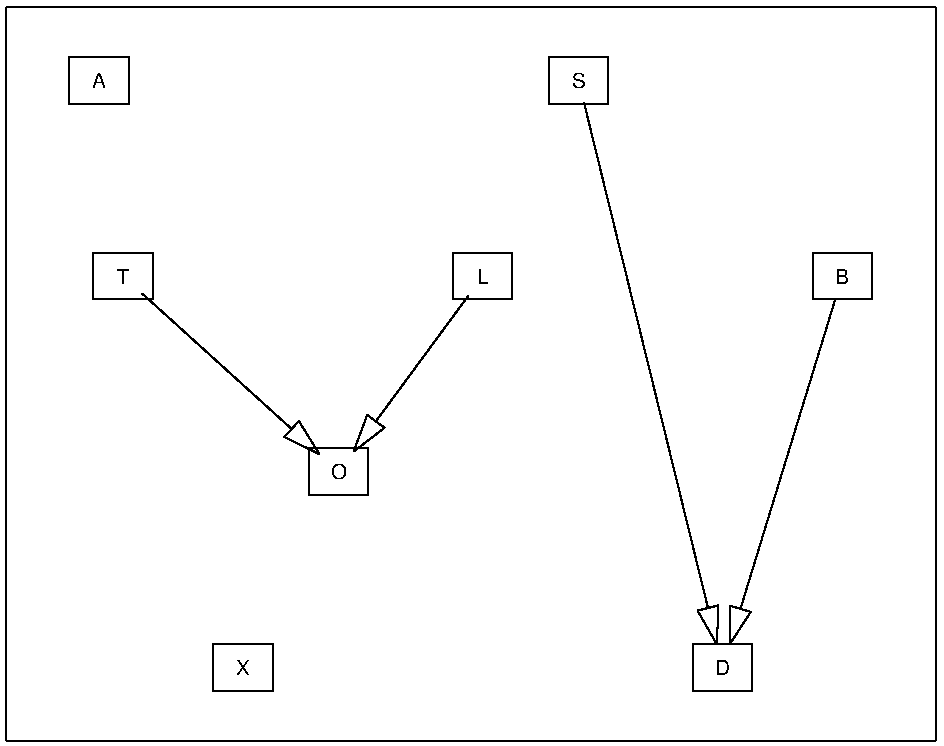
\includegraphics[width=20.3mm, height=14.25mm]{fig/11-Aug-2003-14-06-42-dag-asia500-GES-RES} &
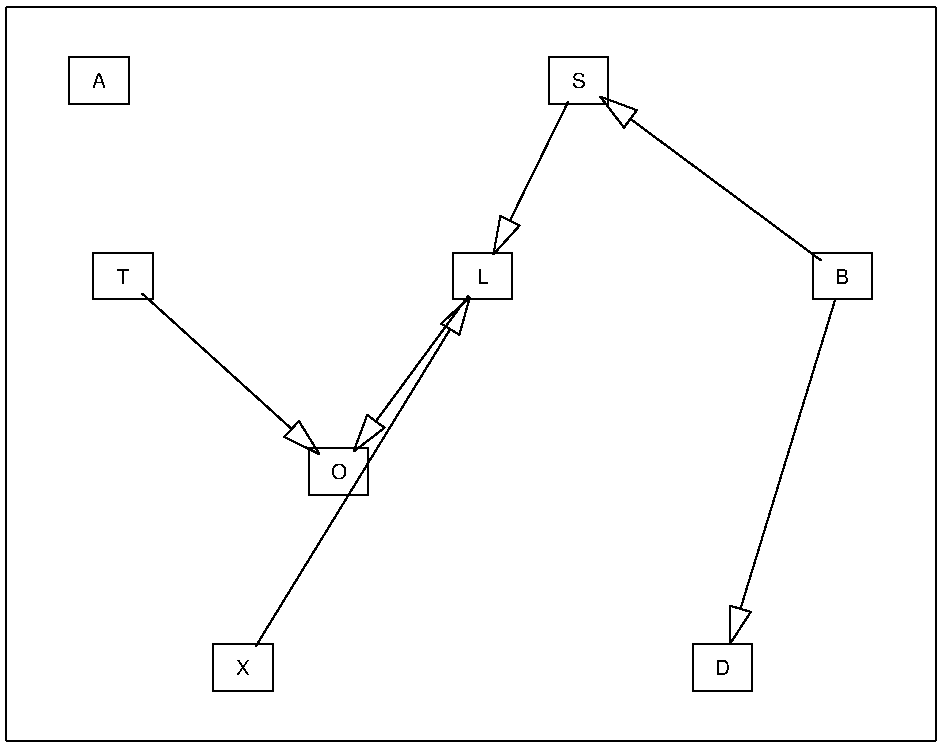
\includegraphics[width=20.3mm, height=14.25mm]{fig/11-Aug-2003-14-06-42-dag-asia1000-GES-RES} &
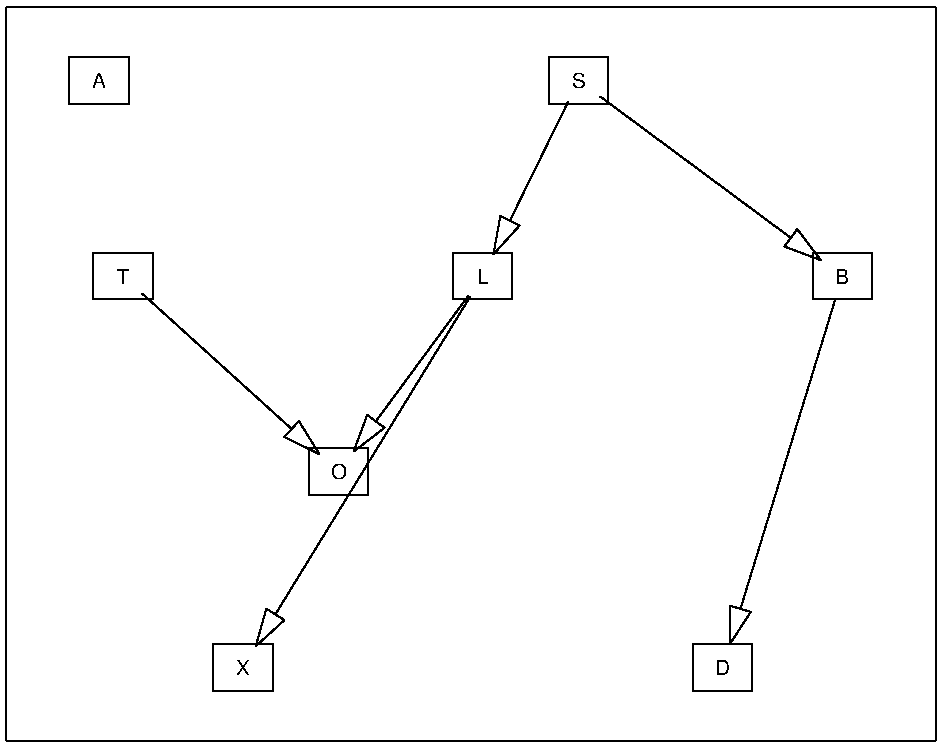
\includegraphics[width=20.3mm, height=14.25mm]{fig/11-Aug-2003-14-06-42-dag-asia2000-GES-RES} &
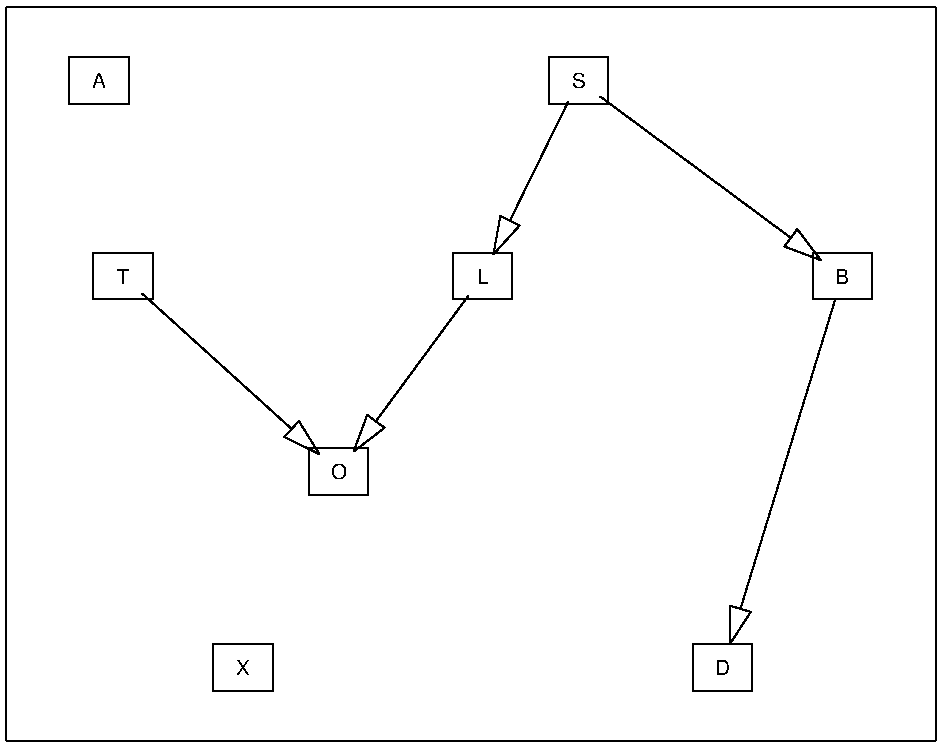
\includegraphics[width=20.3mm, height=14.25mm]{fig/11-Aug-2003-14-06-42-dag-asia5000-GES-RES} &
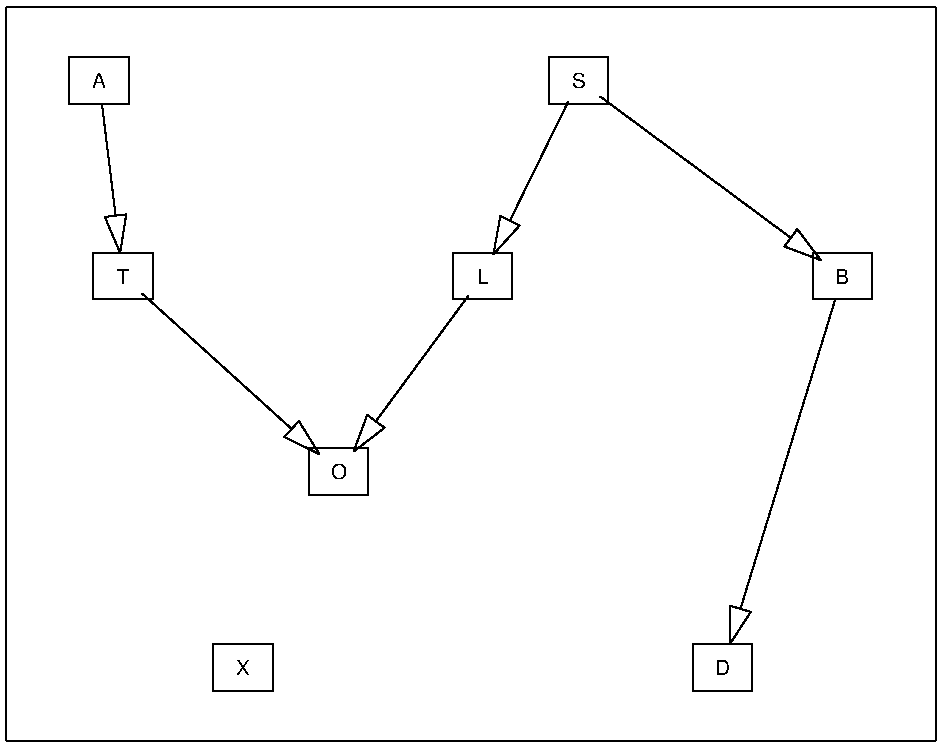
\includegraphics[width=20.3mm, height=14.25mm]{fig/11-Aug-2003-14-06-42-dag-asia10000-GES-RES} &
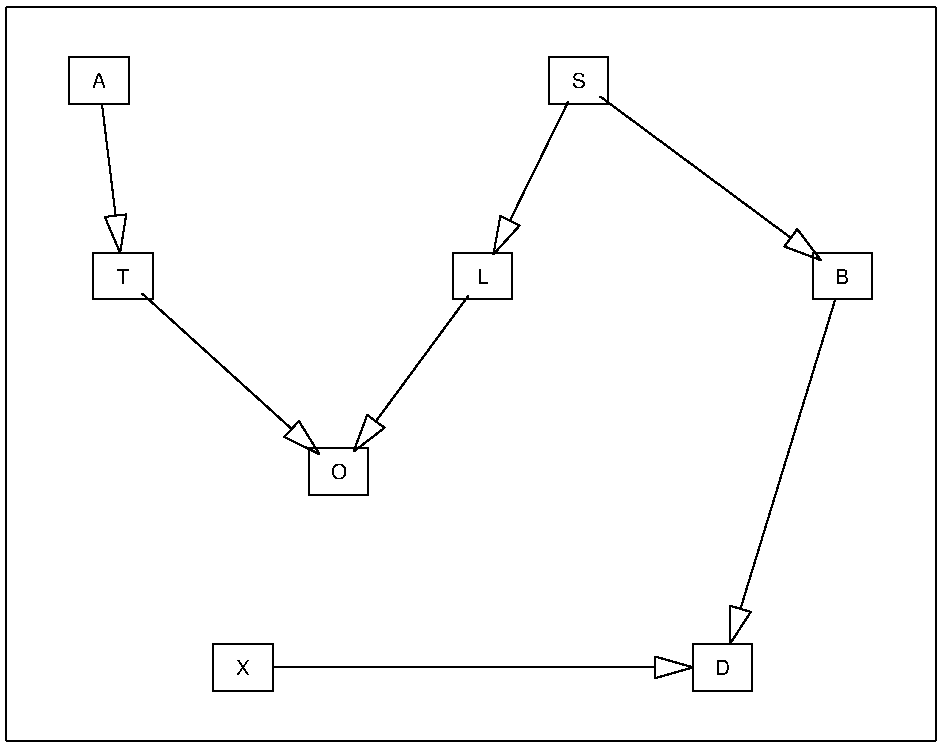
\includegraphics[width=20.3mm, height=14.25mm]{fig/11-Aug-2003-14-06-42-dag-asia15000-GES-RES} \\
& 8;-55765 & 7;-66374 & 6;-61536 & 7;-56386 & 6;-63967 & 5;-63959 & 6;-70154\\
\textsc{bn-pc~} &
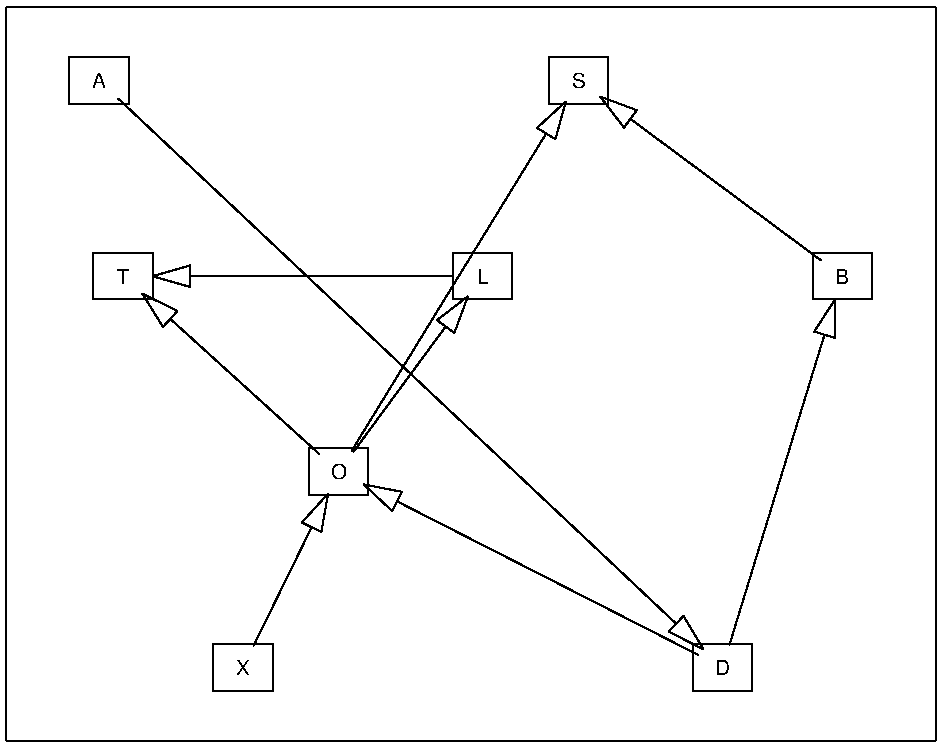
\includegraphics[width=20.3mm, height=14.25mm]{fig/11-Sep-2003-14-37-15-dag-asia250-BNPC-RES} &
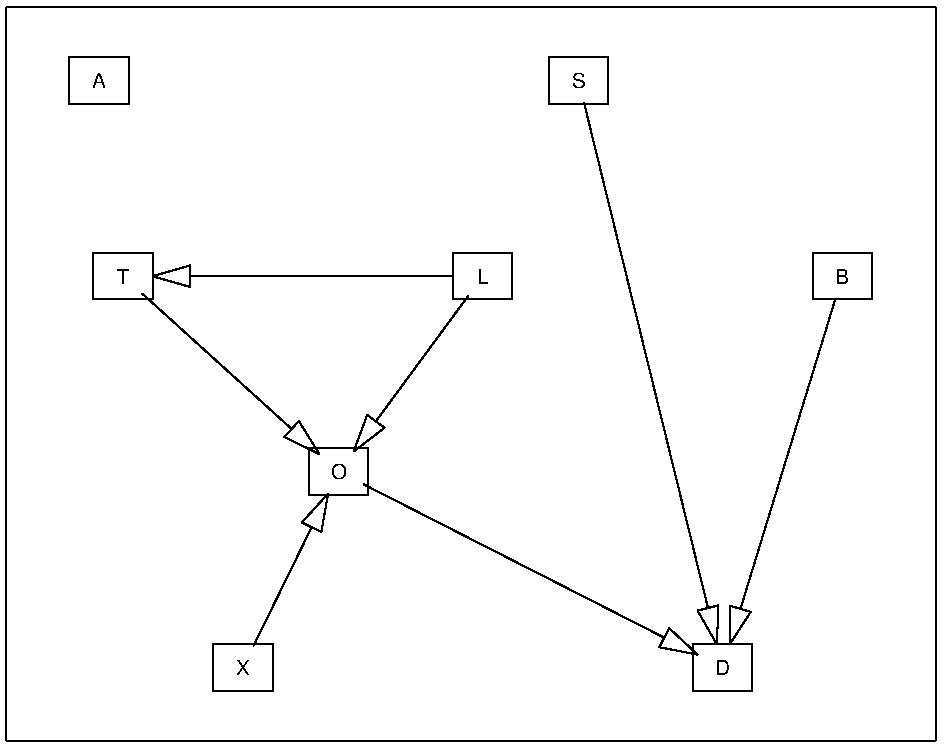
\includegraphics[width=20.3mm, height=14.25mm]{fig/12-Aug-2003-16-26-12-dag-asia500-BNPC-RES} &
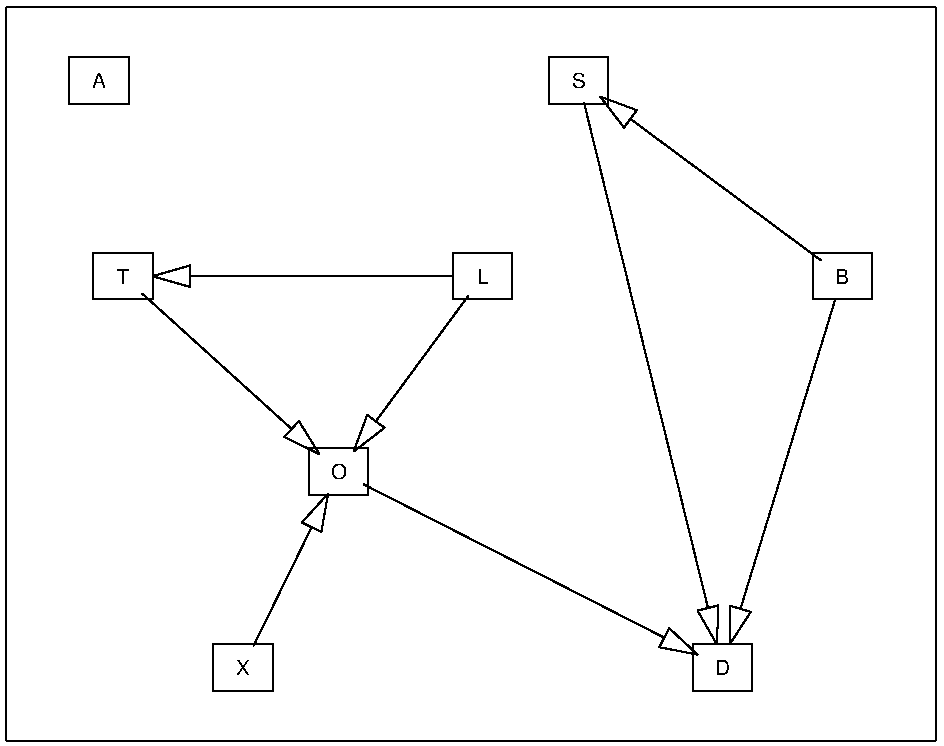
\includegraphics[width=20.3mm, height=14.25mm]{fig/12-Aug-2003-16-26-12-dag-asia1000-BNPC-RES} &
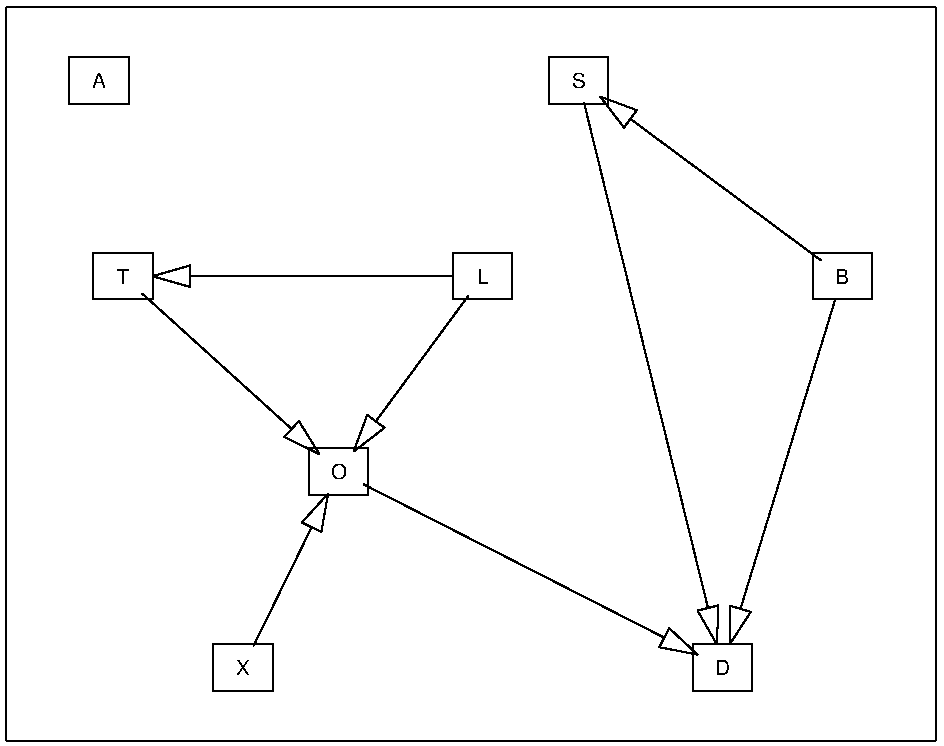
\includegraphics[width=20.3mm, height=14.25mm]{fig/12-Aug-2003-16-26-12-dag-asia2000-BNPC-RES} &
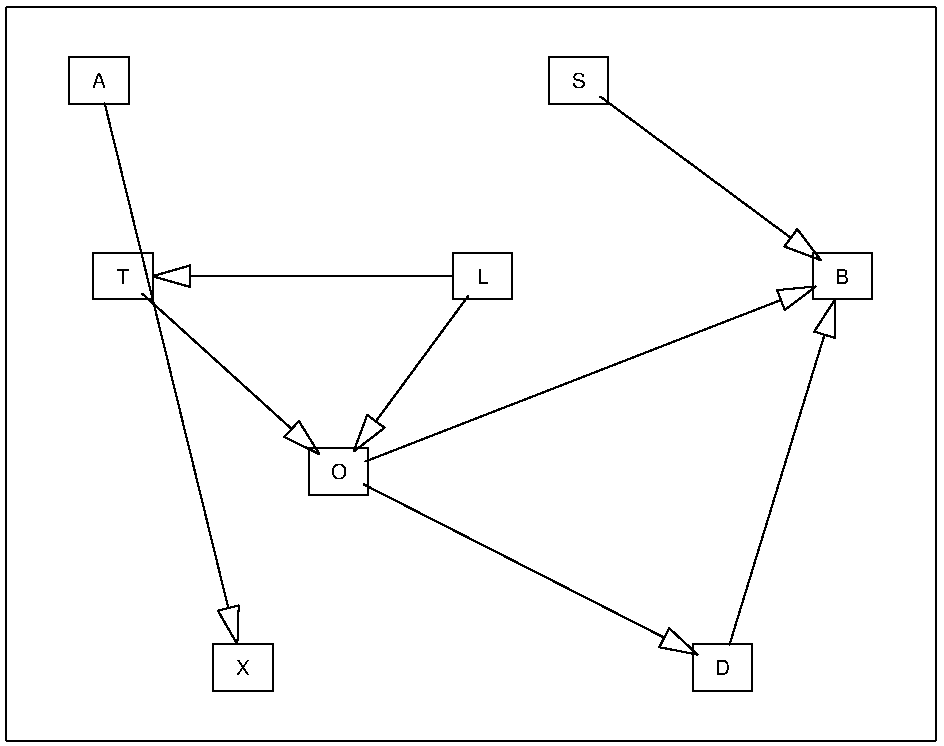
\includegraphics[width=20.3mm, height=14.25mm]{fig/12-Aug-2003-16-34-51-dag-asia5000-BNPC-RES} &
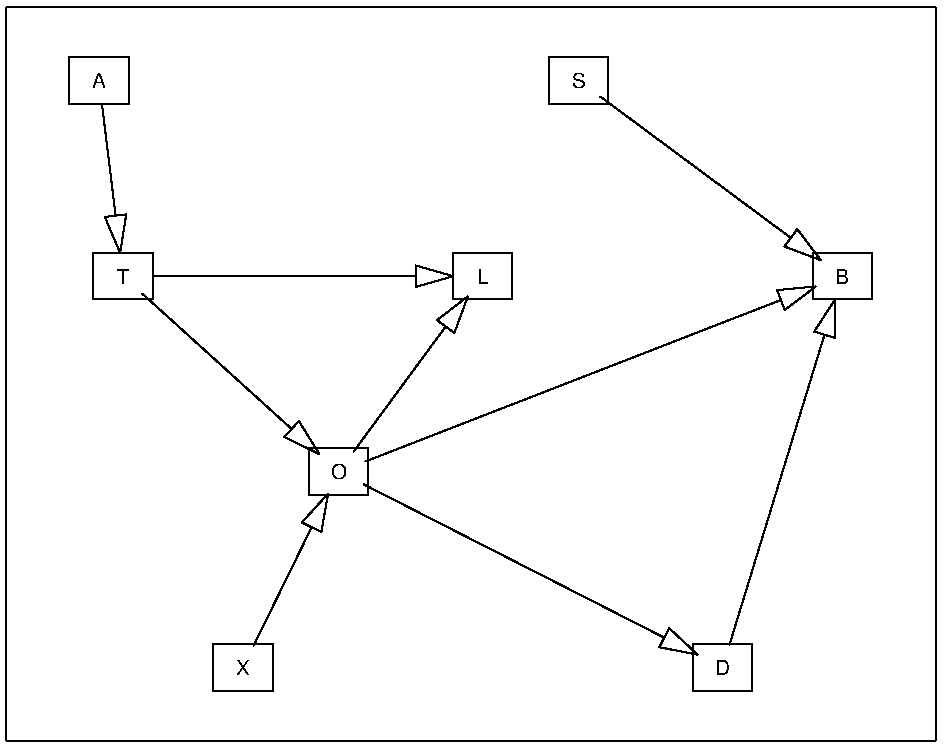
\includegraphics[width=20.3mm, height=14.25mm]{fig/12-Aug-2003-16-41-03-dag-asia10000-BNPC-RES} &
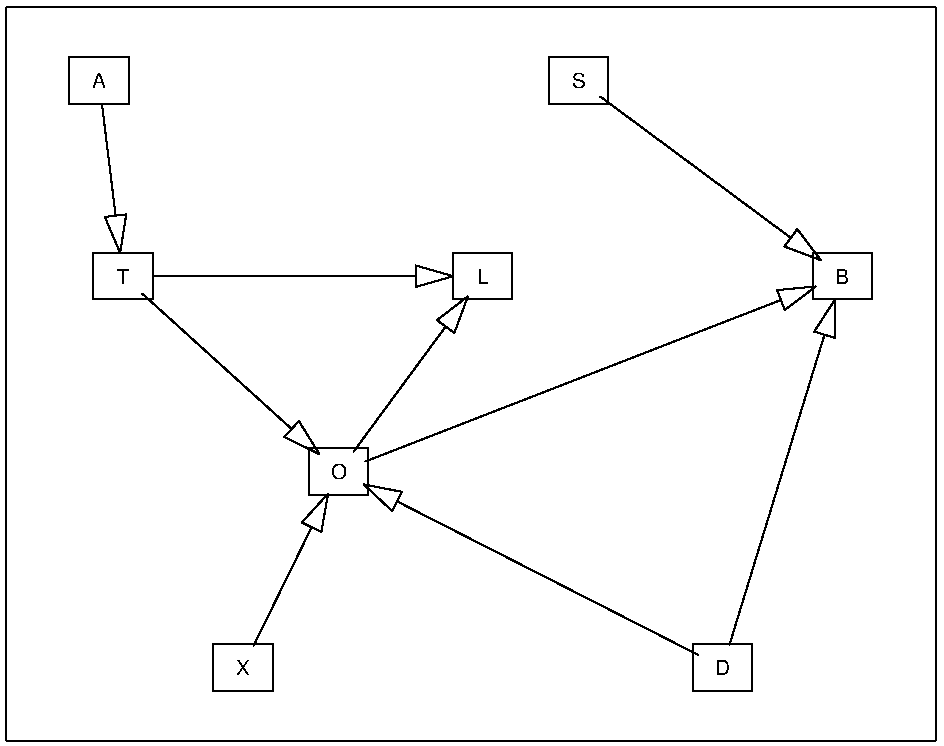
\includegraphics[width=20.3mm, height=14.25mm]{fig/12-Aug-2003-16-41-03-dag-asia15000-BNPC-RES} \\
& 11;-67825 & 6;-73885 & 6;-72529 & 6;-72529 & 7;-73141 & 6;-69046 & 6;-69370\\
\textsc{k2~} &
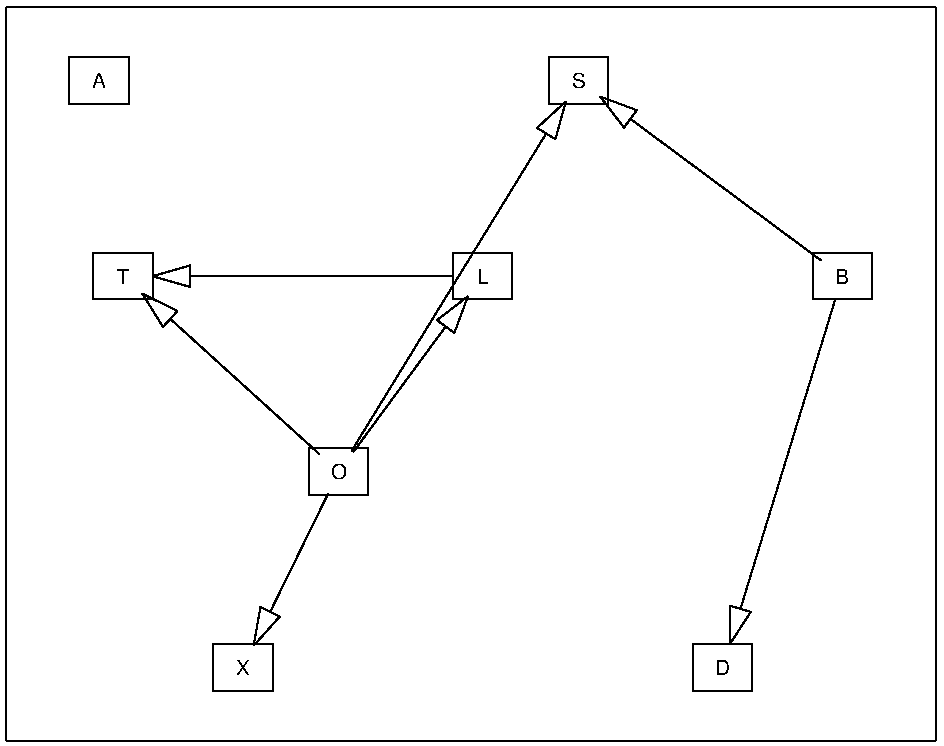
\includegraphics[width=20.3mm, height=14.25mm]{fig/11-Sep-2003-14-28-11-dag-asia250-K2-RES} &
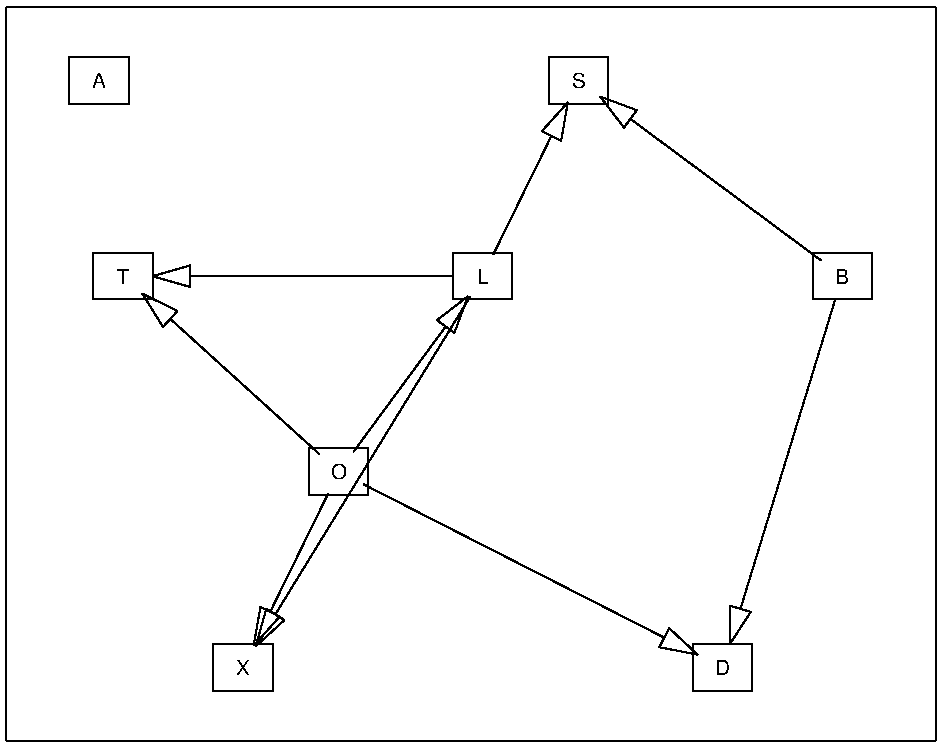
\includegraphics[width=20.3mm, height=14.25mm]{fig/11-Aug-2003-14-51-45-dag-asia500-K2-RES} &
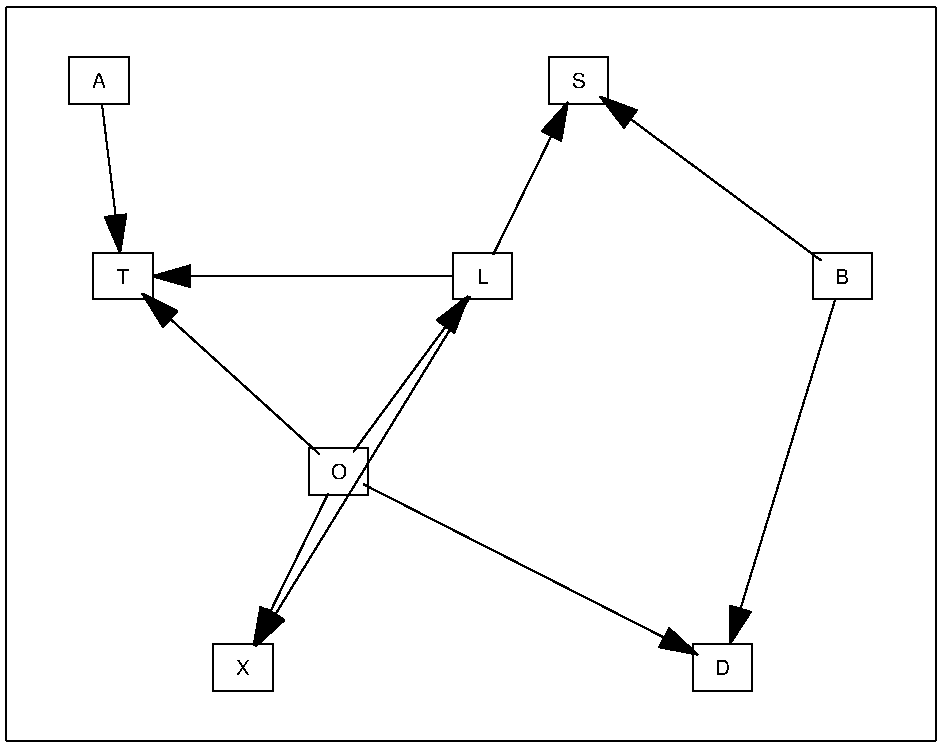
\includegraphics[width=20.3mm, height=14.25mm]{fig/11-Mar-2003-18-40-53-dag-asia1000-K2-RES} &
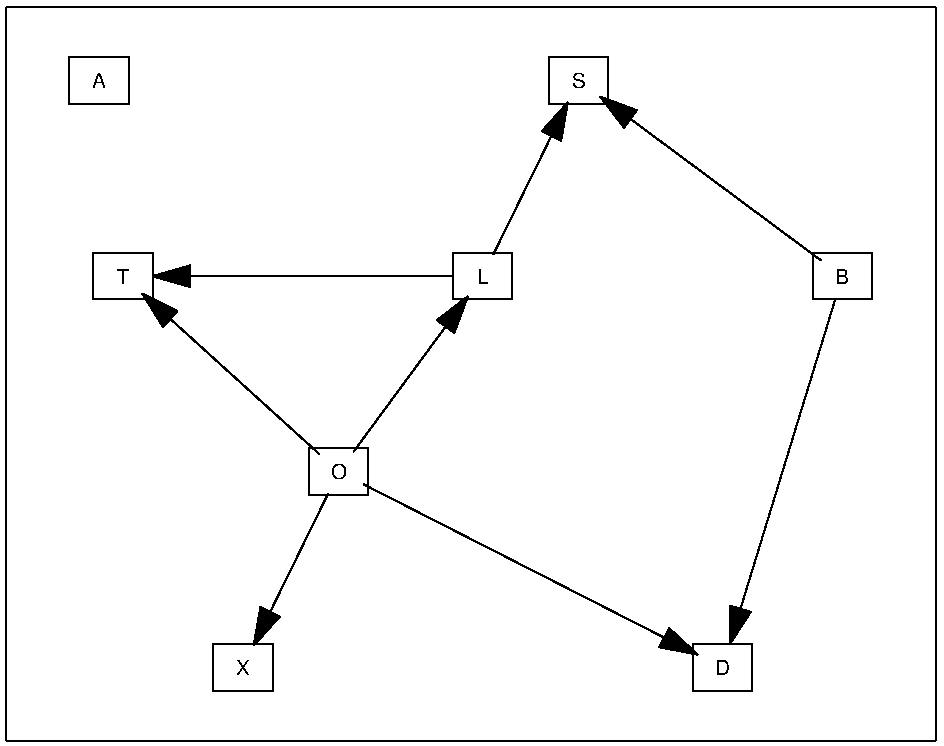
\includegraphics[width=20.3mm, height=14.25mm]{fig/11-Mar-2003-18-40-53-dag-asia2000-K2-RES} &
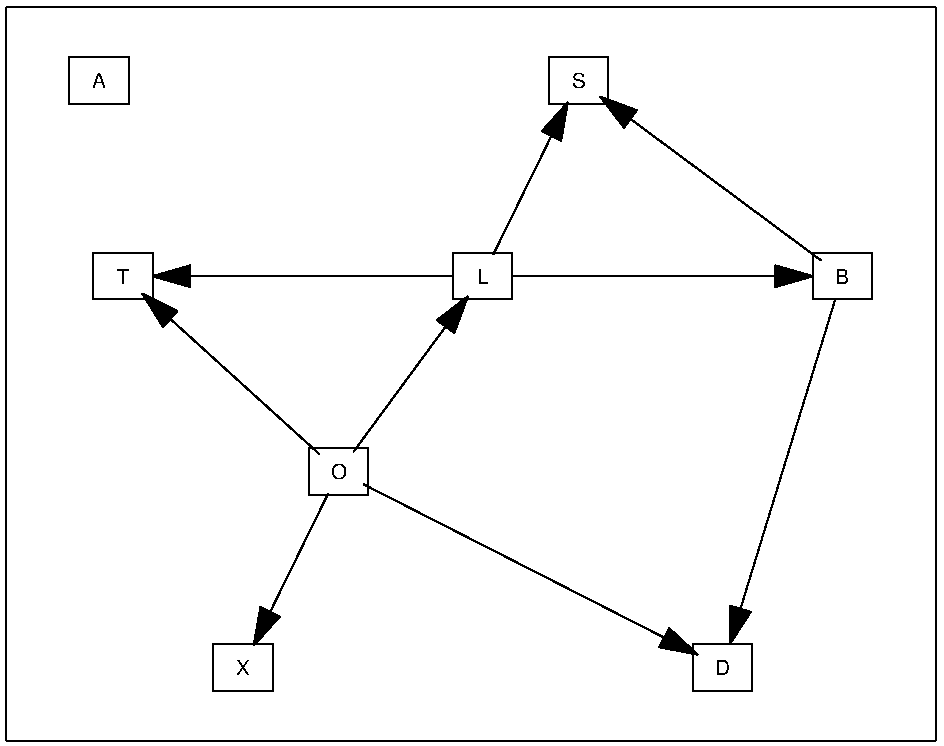
\includegraphics[width=20.3mm, height=14.25mm]{fig/11-Mar-2003-18-40-53-dag-asia5000-K2-RES} &
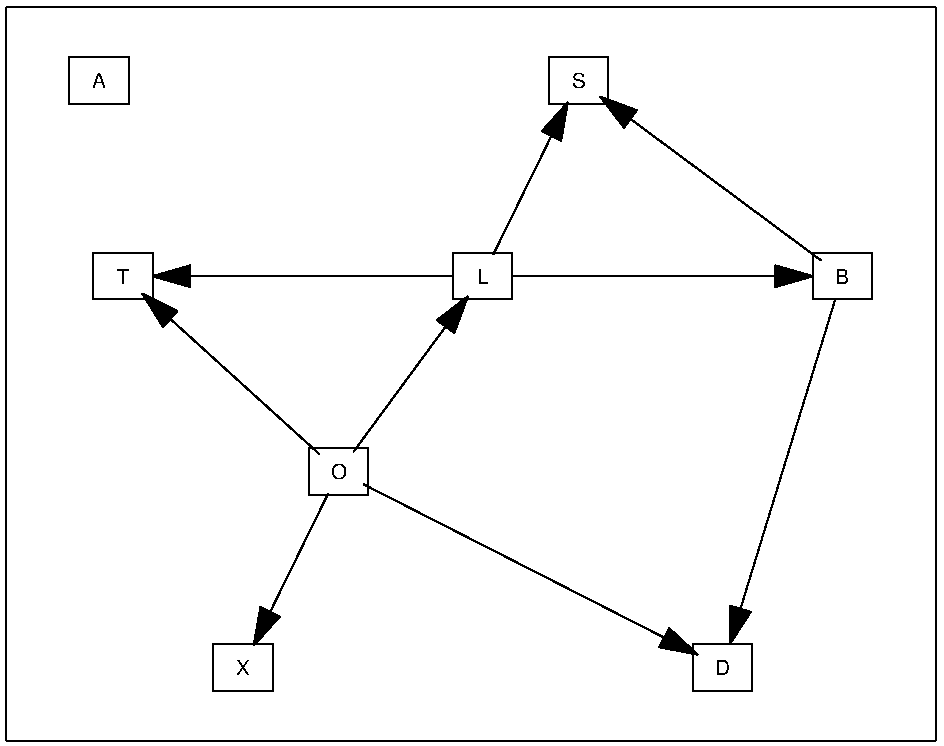
\includegraphics[width=20.3mm, height=14.25mm]{fig/11-Mar-2003-18-40-53-dag-asia10000-K2-RES} &
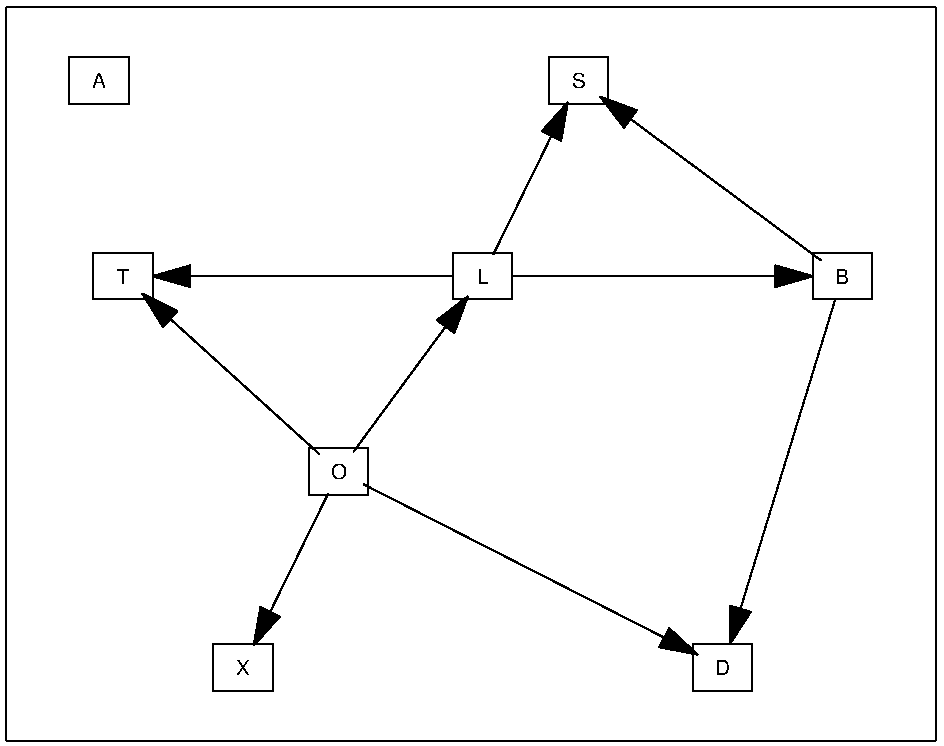
\includegraphics[width=20.3mm, height=14.25mm]{fig/11-Mar-2003-18-40-53-dag-asia15000-K2-RES} \\
& 8;-68141 & 7;-67150 & 6;-67152 & 6;-67147 & 6;-67106 & 6;-67106 & 6;-67106\\
\textsc{k2(2)~} &
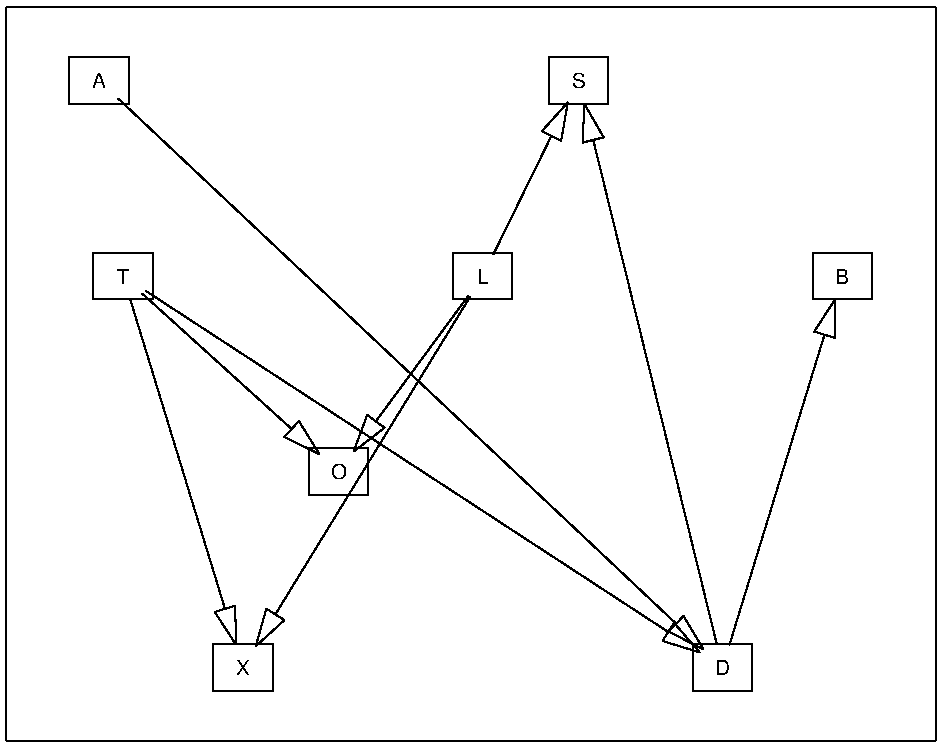
\includegraphics[width=20.3mm, height=14.25mm]{fig/11-Sep-2003-14-47-35-dag-asia250-K2-RES} &
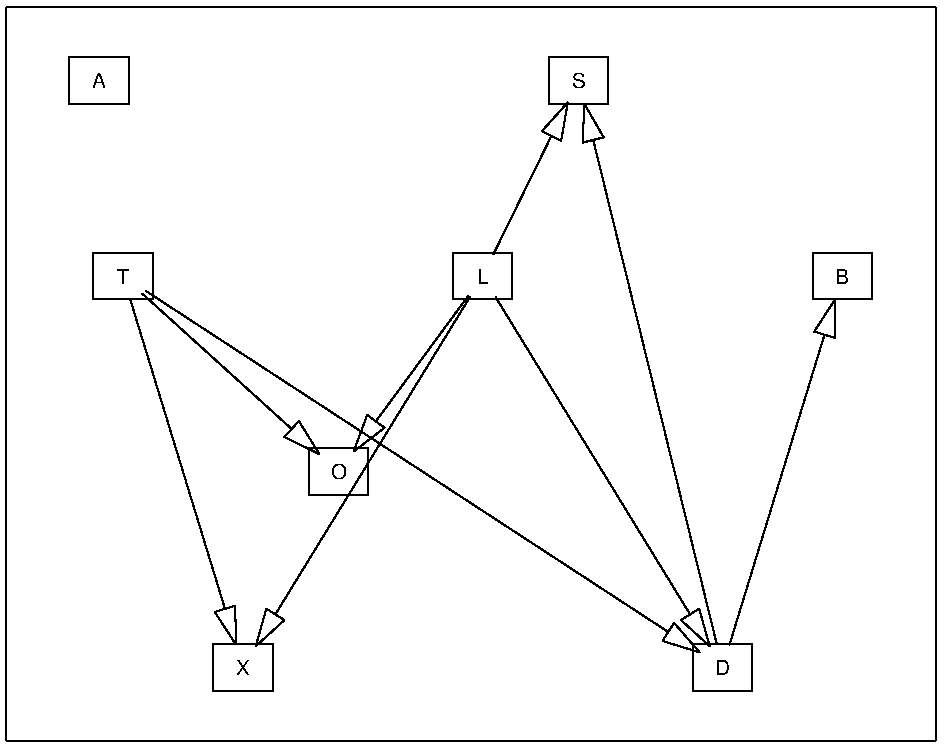
\includegraphics[width=20.3mm, height=14.25mm]{fig/11-Aug-2003-14-59-43-dag-asia500-K2-RES} &
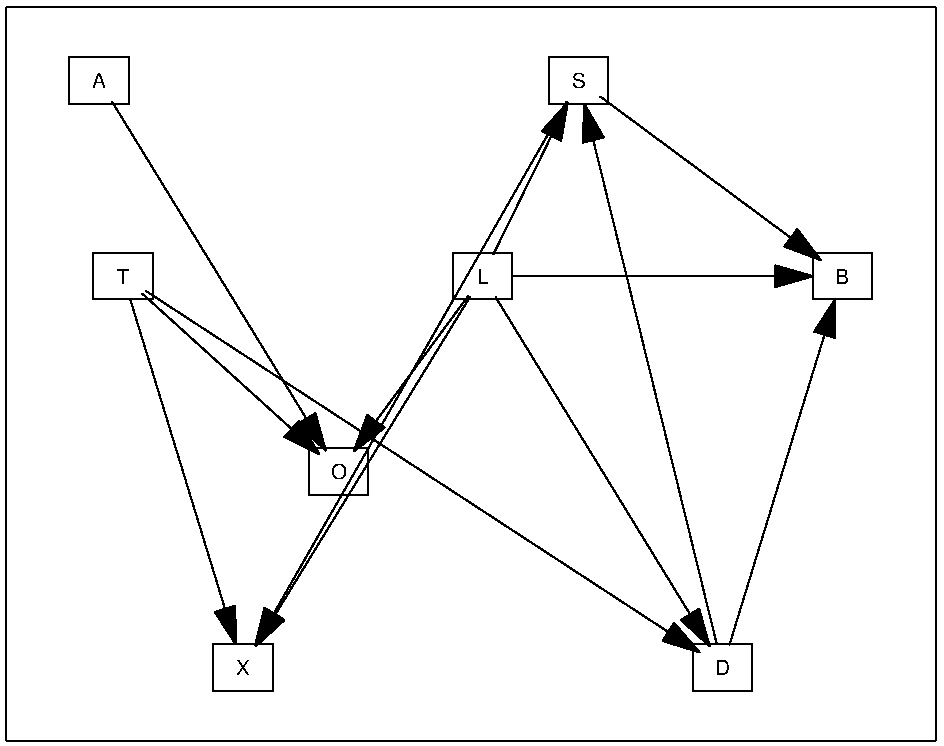
\includegraphics[width=20.3mm, height=14.25mm]{fig/11-Mar-2003-18-46-18-dag-asia1000-K2-RES} &
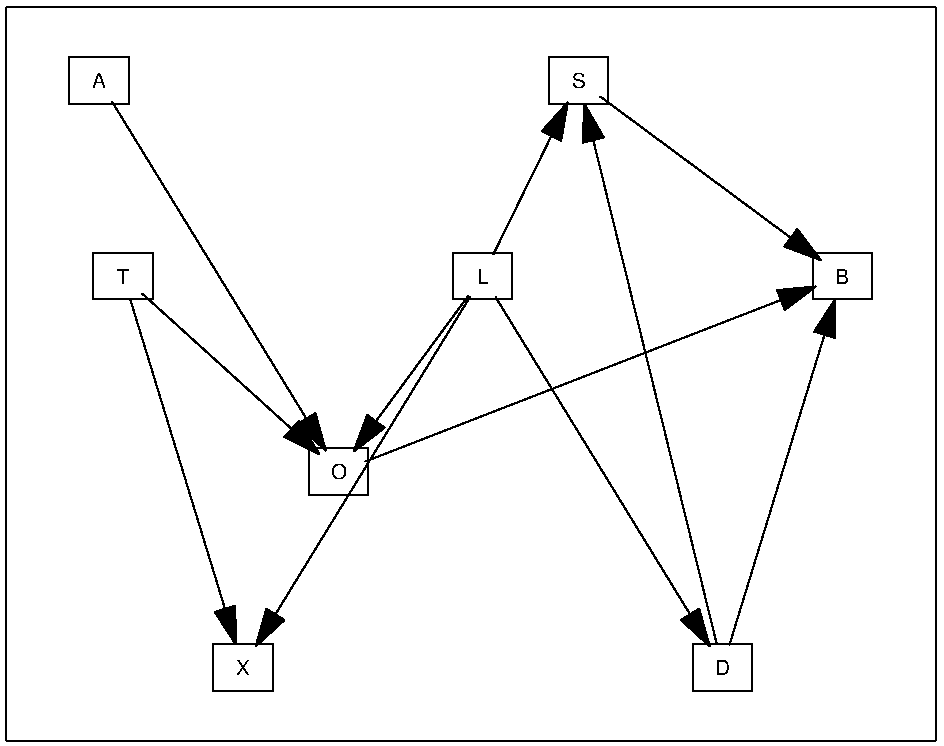
\includegraphics[width=20.3mm, height=14.25mm]{fig/11-Mar-2003-18-46-18-dag-asia2000-K2-RES} &
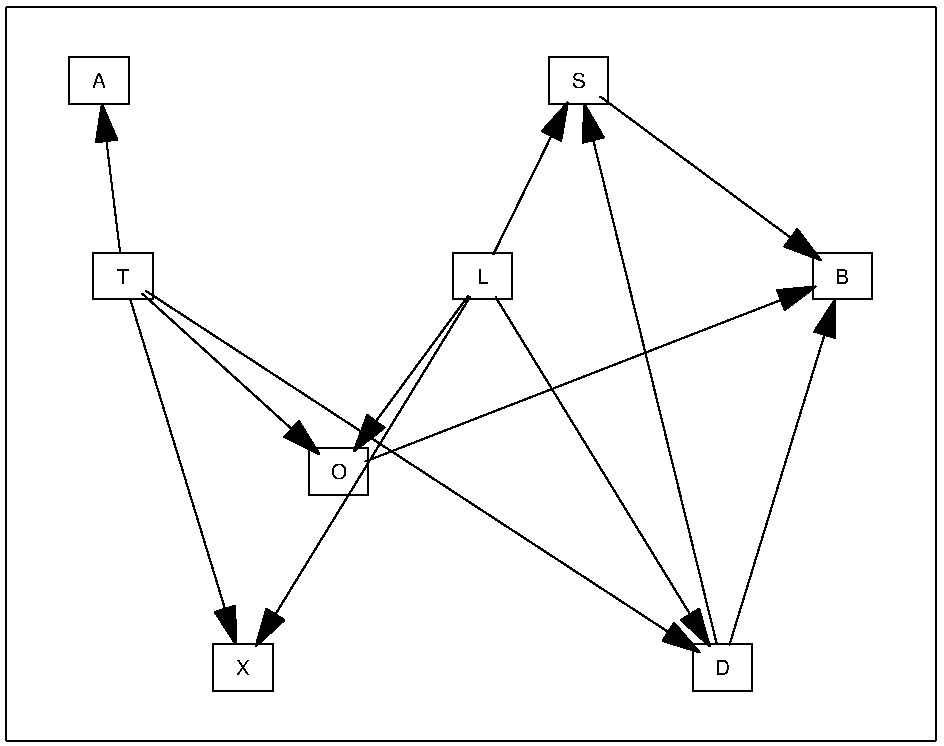
\includegraphics[width=20.3mm, height=14.25mm]{fig/11-Mar-2003-18-46-18-dag-asia5000-K2-RES} &
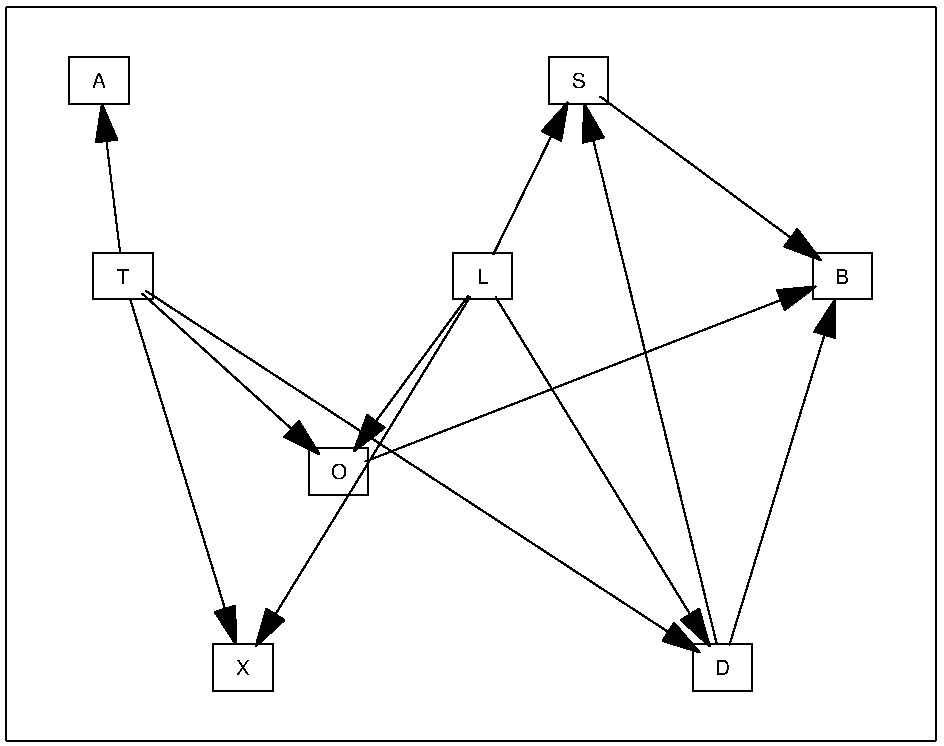
\includegraphics[width=20.3mm, height=14.25mm]{fig/11-Mar-2003-18-46-18-dag-asia10000-K2-RES} &
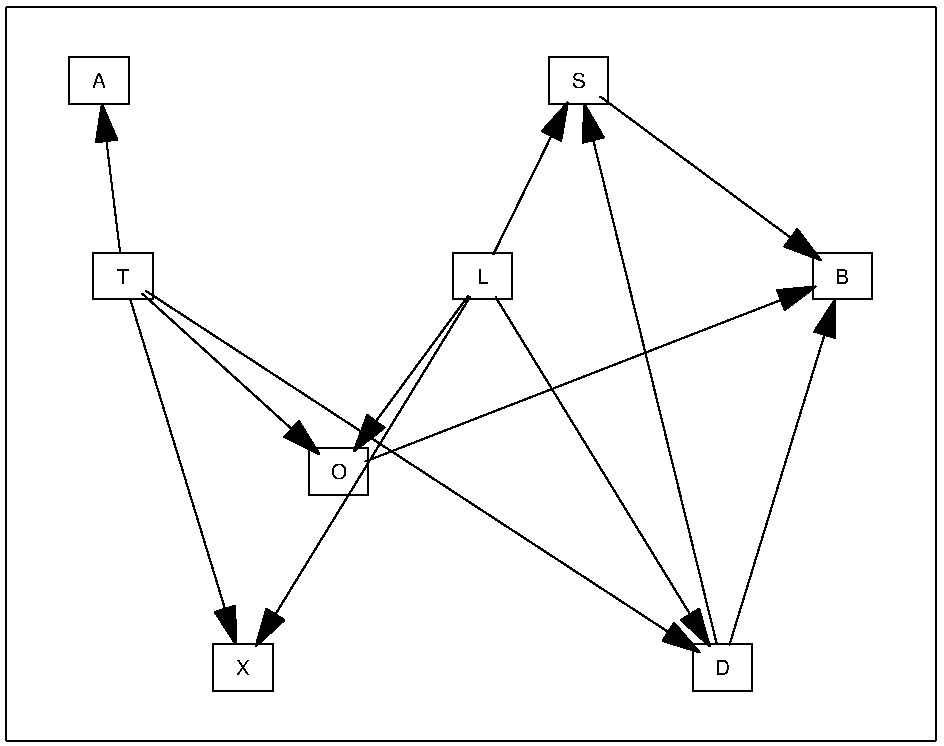
\includegraphics[width=20.3mm, height=14.25mm]{fig/11-Mar-2003-18-46-18-dag-asia15000-K2-RES} \\
& 11;-68643 & 11;-68089 & 11;-67221 & 10;-67216 & 9;-67129 & 9;-67129 & 9;-67129\\
\textsc{k2+t~} &
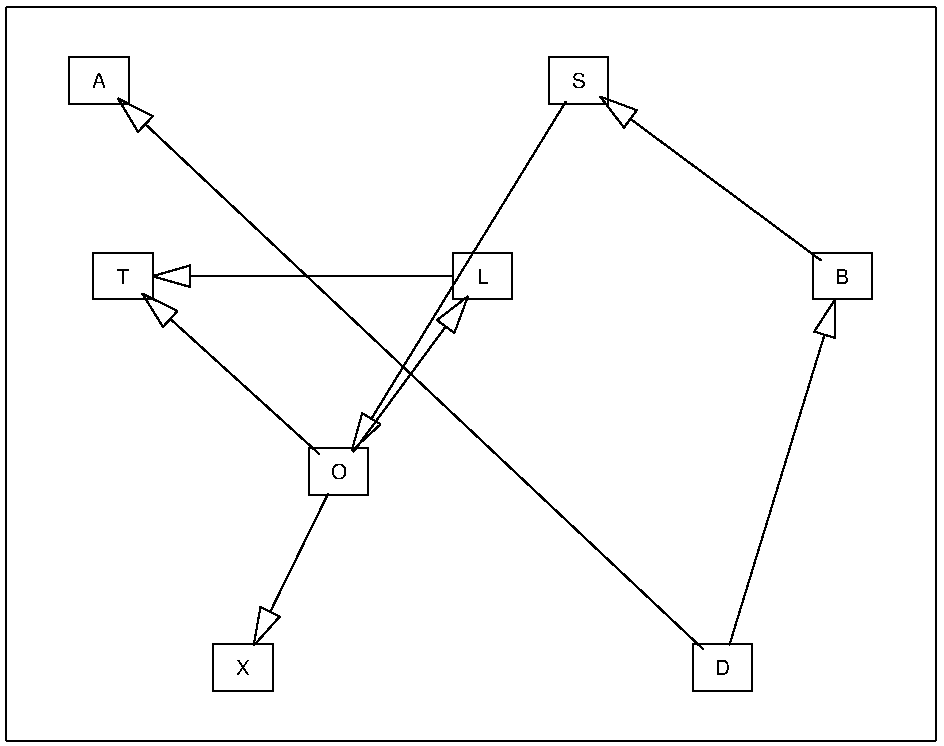
\includegraphics[width=20.3mm, height=14.25mm]{fig/11-Sep-2003-14-28-11-dag-asia250-K2+MSWT-RES} &
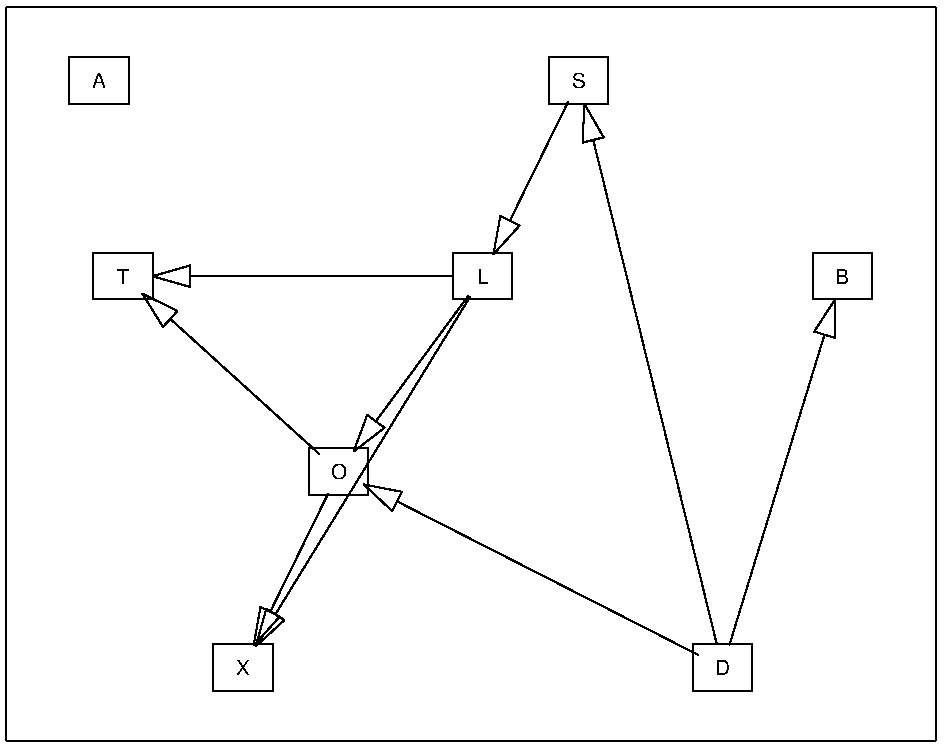
\includegraphics[width=20.3mm, height=14.25mm]{fig/11-Aug-2003-14-51-45-dag-asia500-K2+MSWT-RES} &
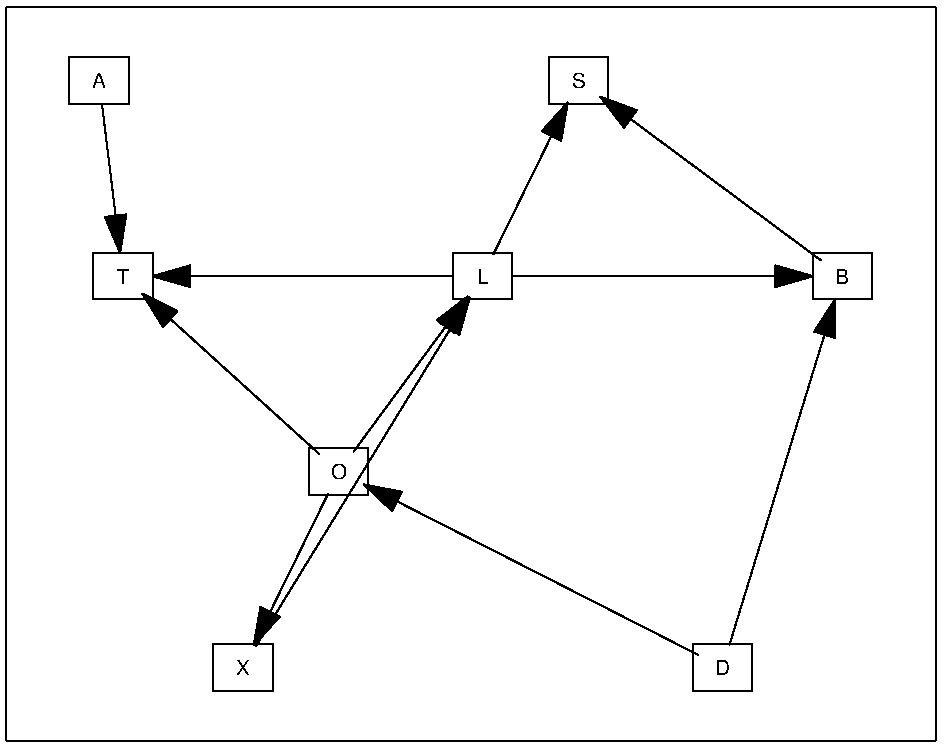
\includegraphics[width=20.3mm, height=14.25mm]{fig/11-Mar-2003-18-40-53-dag-asia1000-K2+MSWT-RES} &
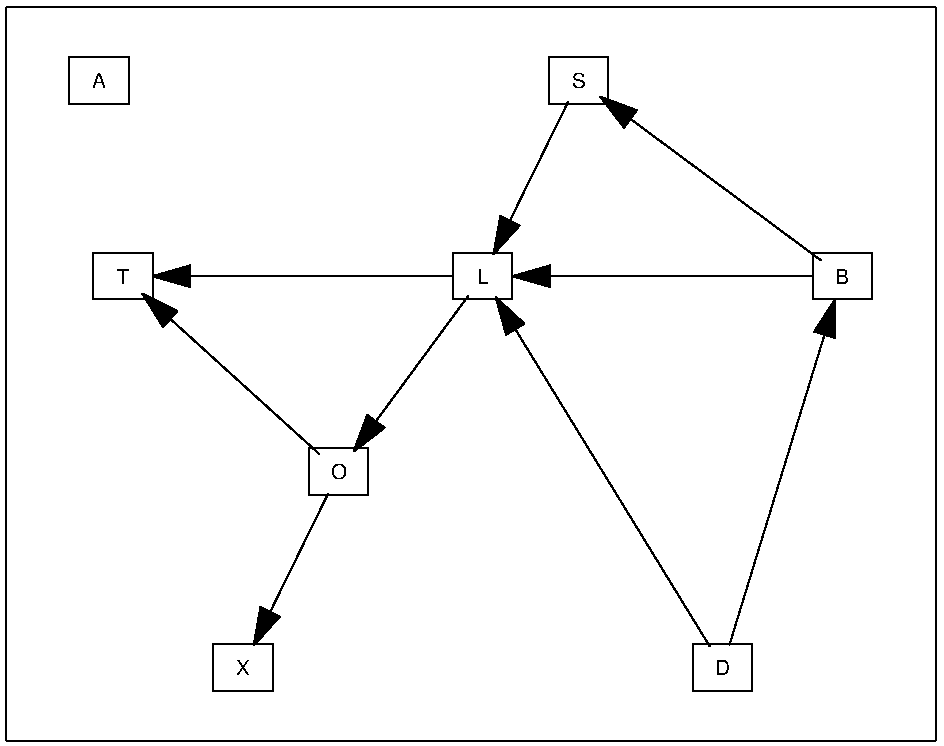
\includegraphics[width=20.3mm, height=14.25mm]{fig/11-Mar-2003-18-40-53-dag-asia2000-K2+MSWT-RES} &
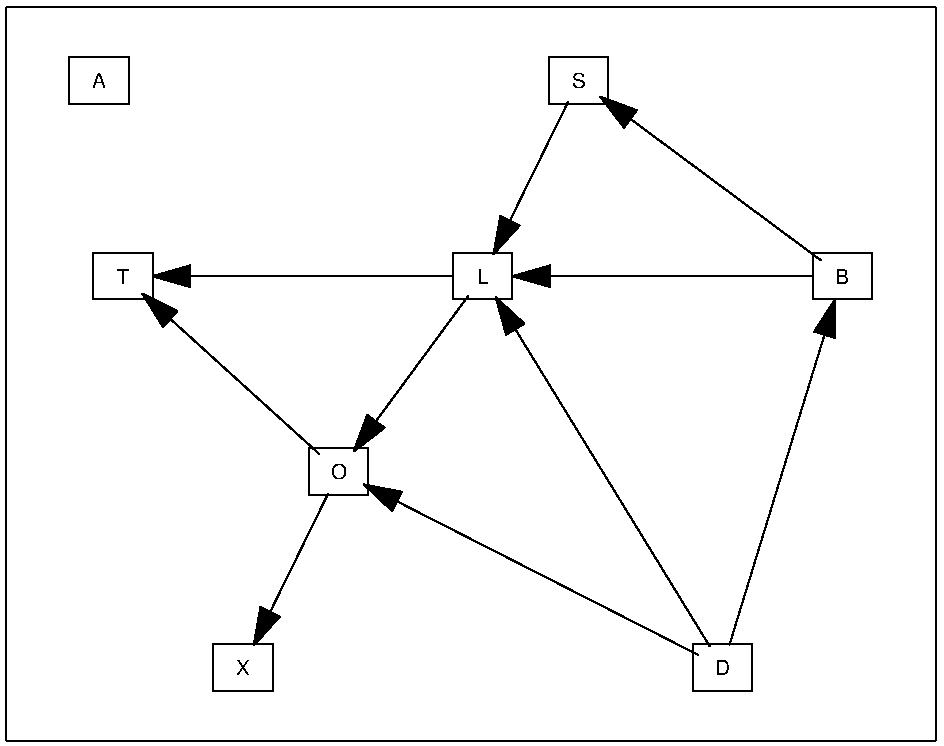
\includegraphics[width=20.3mm, height=14.25mm]{fig/11-Mar-2003-18-40-53-dag-asia5000-K2+MSWT-RES} &
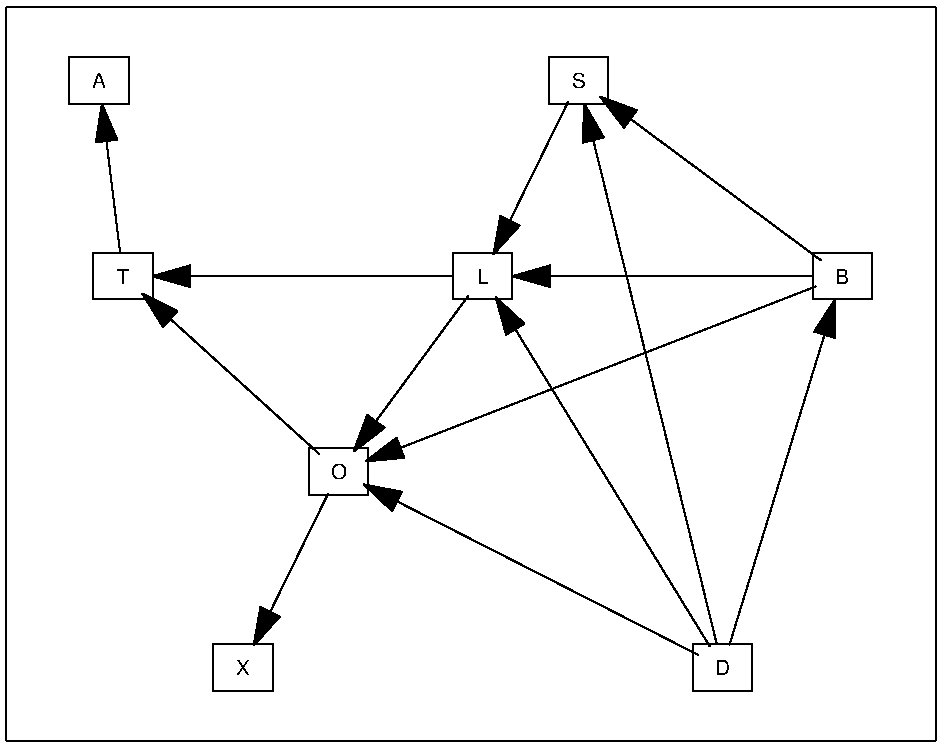
\includegraphics[width=20.3mm, height=14.25mm]{fig/11-Mar-2003-18-40-53-dag-asia10000-K2+MSWT-RES} &
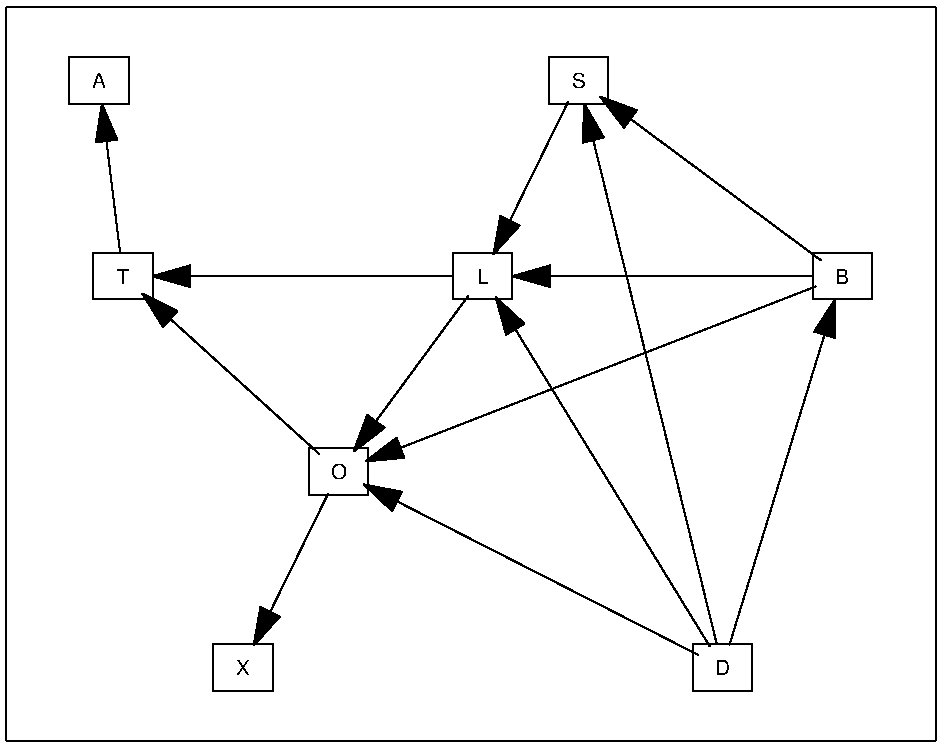
\includegraphics[width=20.3mm, height=14.25mm]{fig/11-Mar-2003-18-40-53-dag-asia15000-K2+MSWT-RES} \\
& 10;-68100 & 8;-68418 & 9;-67185 & 8;-67317 & 8;-67236 & 10;-67132 & 10;-67132\\
\textsc{k2-t~} &
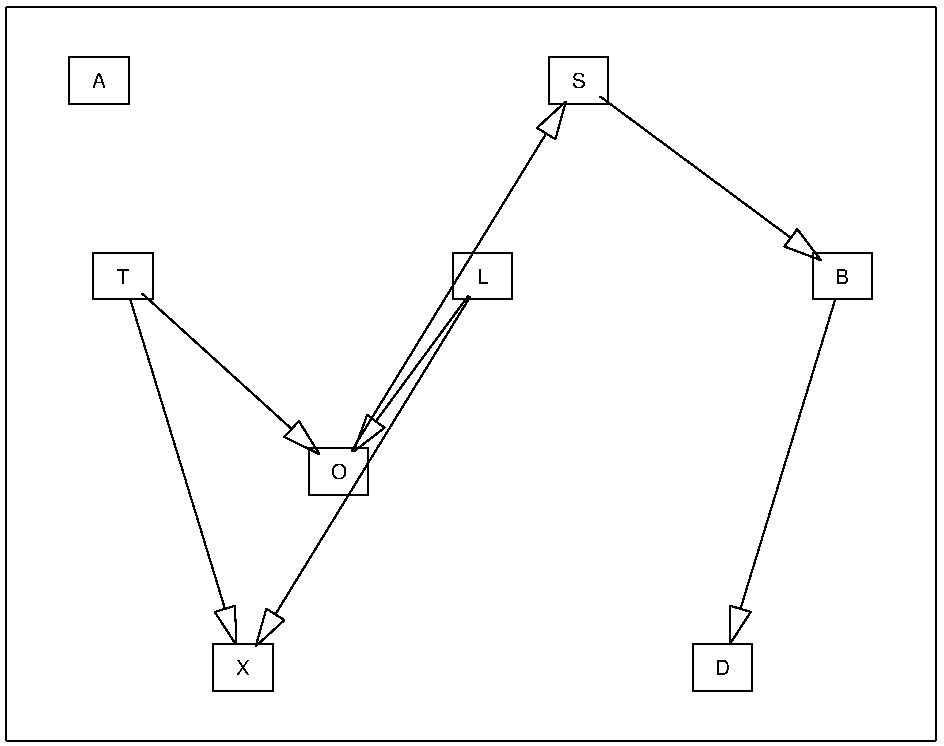
\includegraphics[width=20.3mm, height=14.25mm]{fig/11-Sep-2003-14-47-35-dag-asia250-K2-MSWT-RES} &
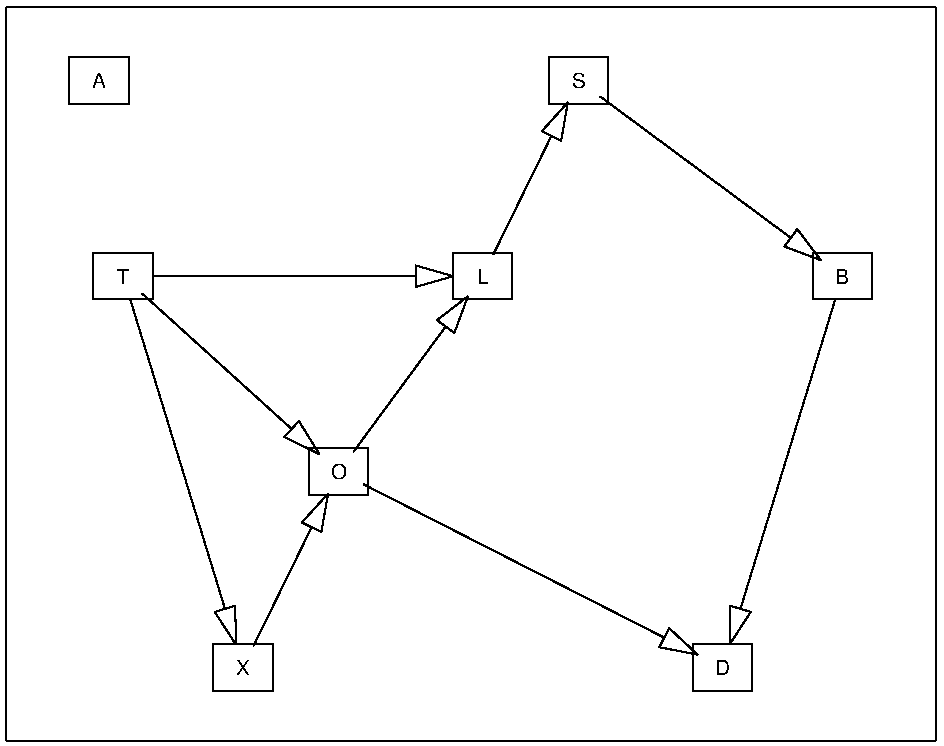
\includegraphics[width=20.3mm, height=14.25mm]{fig/11-Aug-2003-14-59-43-dag-asia500-K2-MSWT-RES} &
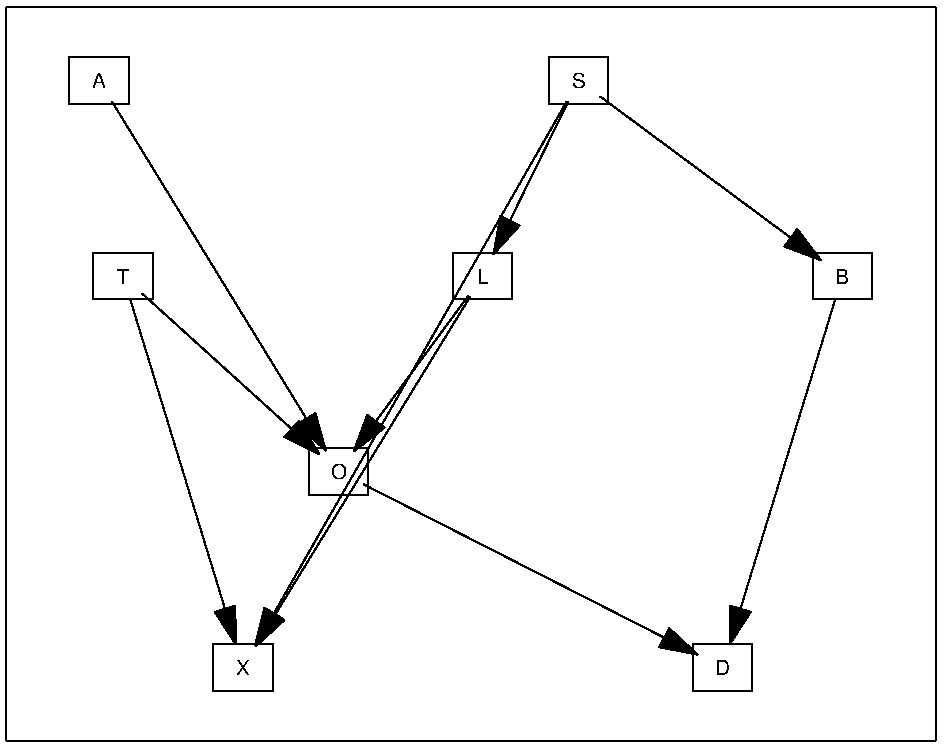
\includegraphics[width=20.3mm, height=14.25mm]{fig/11-Mar-2003-18-46-18-dag-asia1000-K2-MSWT-RES} &
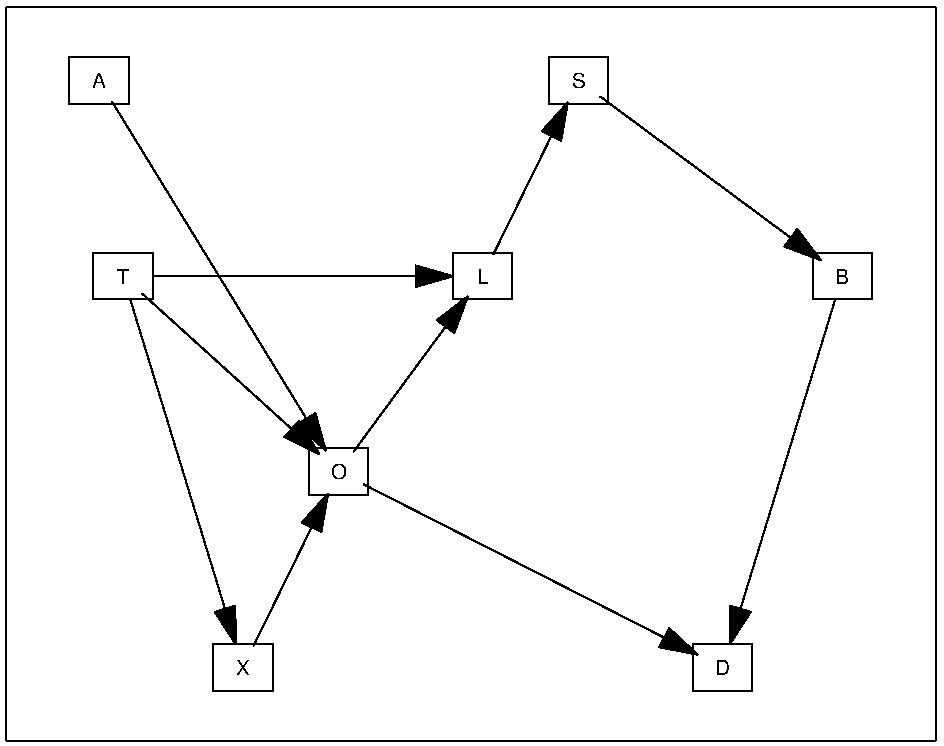
\includegraphics[width=20.3mm, height=14.25mm]{fig/11-Mar-2003-18-46-18-dag-asia2000-K2-MSWT-RES} &
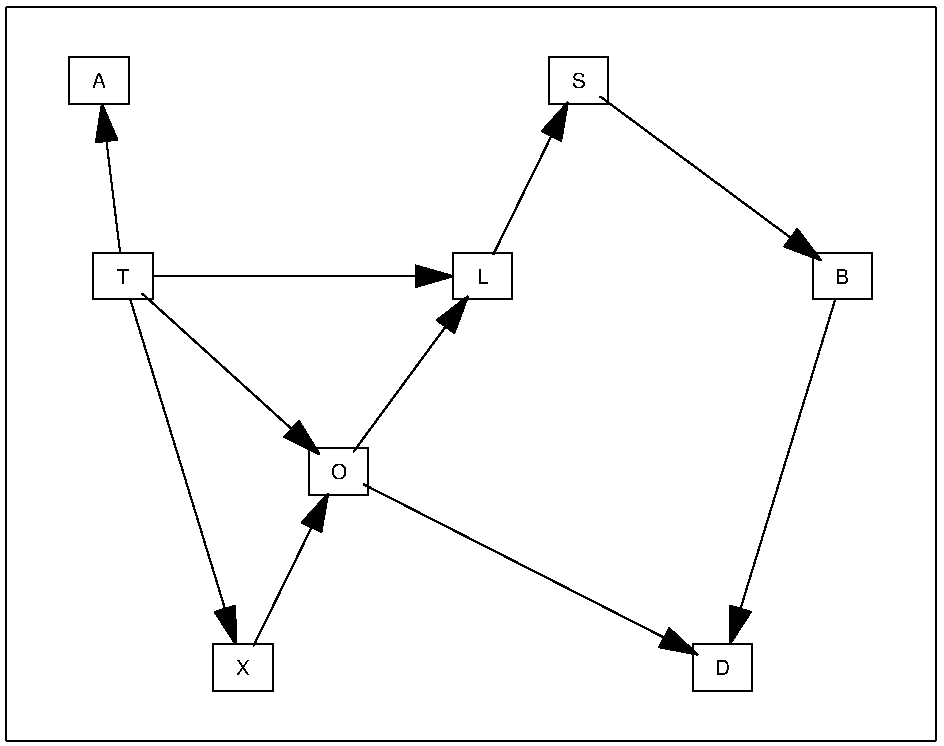
\includegraphics[width=20.3mm, height=14.25mm]{fig/11-Mar-2003-18-46-18-dag-asia5000-K2-MSWT-RES} &
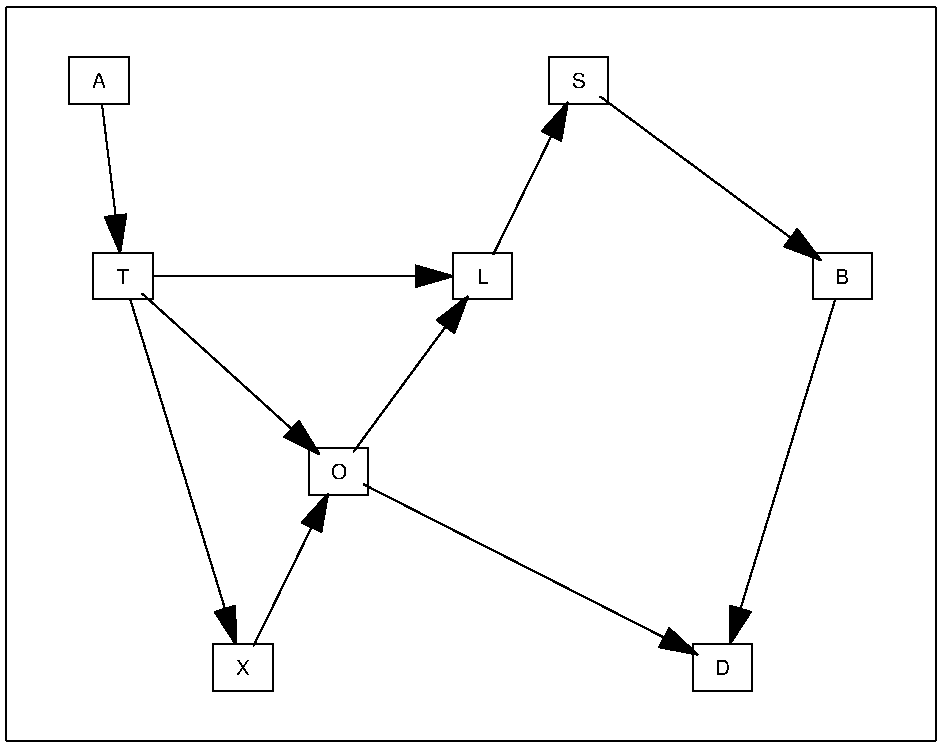
\includegraphics[width=20.3mm, height=14.25mm]{fig/11-Mar-2003-18-46-18-dag-asia10000-K2-MSWT-RES} &
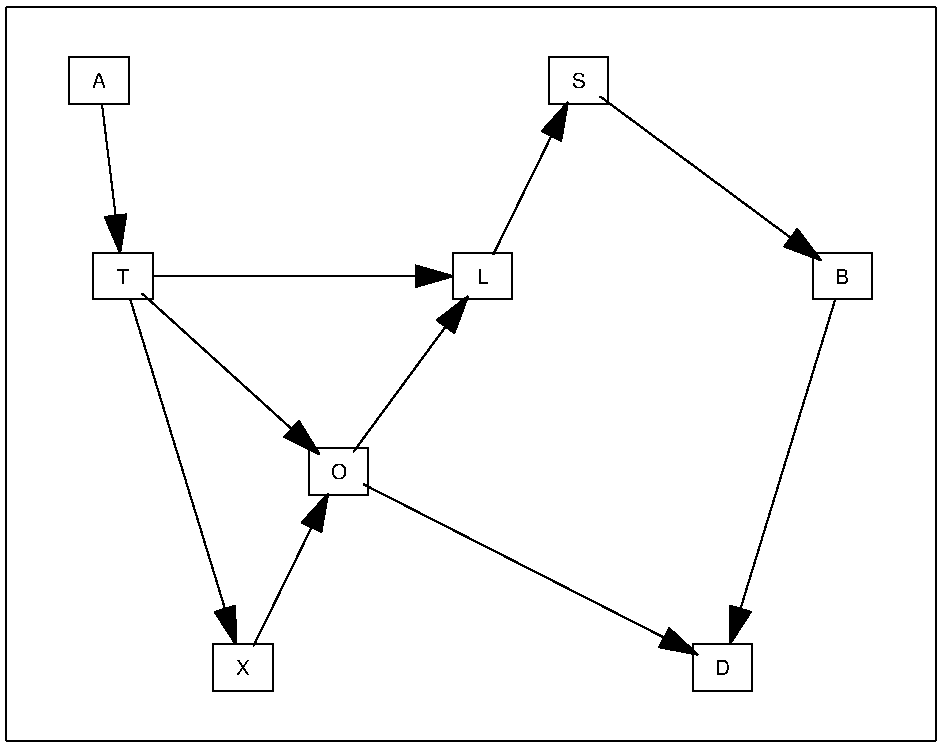
\includegraphics[width=20.3mm, height=14.25mm]{fig/11-Mar-2003-18-46-18-dag-asia15000-K2-MSWT-RES} \\
& 7;-68097 & 6;-67099 & 6;-67112 & 7;-67105 & 6;-67091 & 5;-67091 & 5;-67091\\
\textsc{gs-0~} &
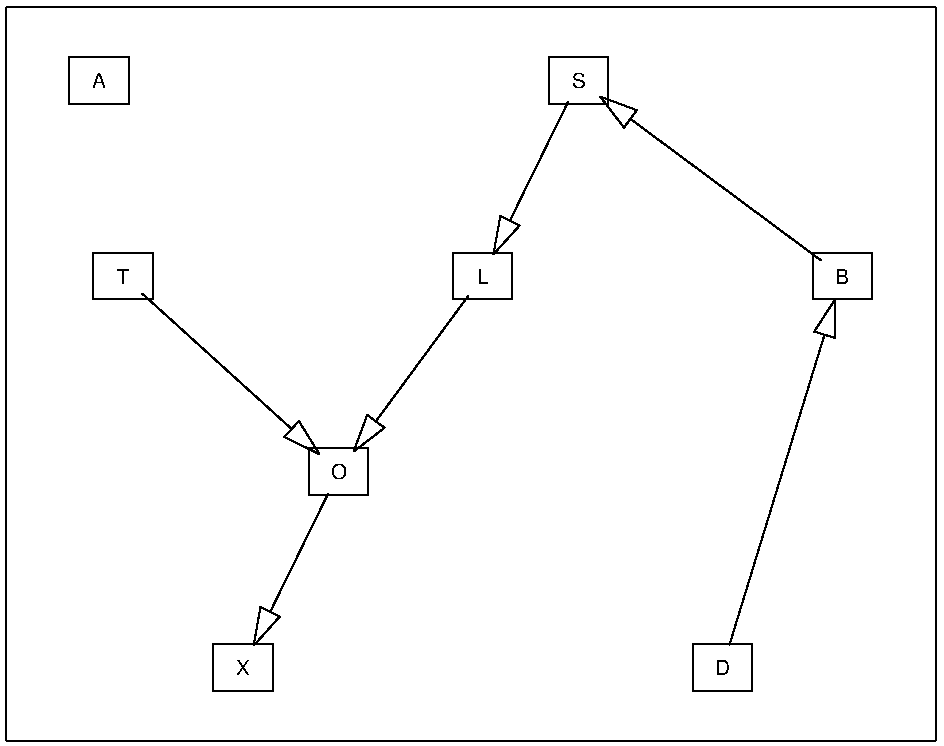
\includegraphics[width=20.3mm, height=14.25mm]{fig/11-Sep-2003-14-39-38-dag-asia250-GS-RES} &
\includegraphics[width=20.3mm, height=14.25mm]{fig/11-Aug-2003-15-08-57-dag-asia500-GS-RES} &
\includegraphics[width=20.3mm, height=14.25mm]{fig/26-Feb-2003-16-33-13-dag-asia1000-GS-RES} &
\includegraphics[width=20.3mm, height=14.25mm]{fig/26-Feb-2003-16-33-13-dag-asia2000-GS-RES} &
\includegraphics[width=20.3mm, height=14.25mm]{fig/26-Feb-2003-16-33-13-dag-asia5000-GS-RES} &
\includegraphics[width=20.3mm, height=14.25mm]{fig/26-Feb-2003-16-33-13-dag-asia10000-GS-RES} &
\includegraphics[width=20.3mm, height=14.25mm]{fig/26-Feb-2003-16-33-13-dag-asia15000-GS-RES} \\
& 4;-67961 & 9;-68081 & 2;-67093 & 5;-67096 & 7;-67128 & 9;-67132 & 8;-67104 \\
\textsc{gs+t~} &
\includegraphics[width=20.3mm, height=14.25mm]{fig/11-Sep-2003-14-39-38-dag-asia250-GS-MSWT-RES} &
\includegraphics[width=20.3mm, height=14.25mm]{fig/11-Aug-2003-15-08-57-dag-asia500-GS-MSWT-RES} &
\includegraphics[width=20.3mm, height=14.25mm]{fig/26-Feb-2003-16-33-13-dag-asia1000-GS-MSWT-RES} &
\includegraphics[width=20.3mm, height=14.25mm]{fig/26-Feb-2003-16-33-13-dag-asia2000-GS-MSWT-RES} &
\includegraphics[width=20.3mm, height=14.25mm]{fig/26-Feb-2003-16-33-13-dag-asia5000-GS-MSWT-RES} &
\includegraphics[width=20.3mm, height=14.25mm]{fig/26-Feb-2003-16-33-13-dag-asia10000-GS-MSWT-RES} &
\colorbox{Ocase}{\includegraphics[width=20.3mm, height=14.25mm]{fig/26-Feb-2003-16-33-13-dag-asia15000-GS-MSWT-RES}} \\
& 9;-68096 & 6;-68415 & 2;-67093 & 7;-67262 & 2;-67093 & 2;-67093 & \colorbox{Ocase}{1;-67086~~~} \\
\textsc{ges~} &
\includegraphics[width=20.3mm, height=14.25mm]{fig/11-Sep-2003-14-43-10-dag-asia250-GES-RES} &
\includegraphics[width=20.3mm, height=14.25mm]{fig/11-Aug-2003-13-36-32-dag-asia500-GES-RES} &
\includegraphics[width=20.3mm, height=14.25mm]{fig/28-Jul-2003-17-49-38-dag-asia1000-GES-RES} &
\includegraphics[width=20.3mm, height=14.25mm]{fig/28-Jul-2003-17-49-38-dag-asia2000-GES-RES} &
\colorbox{Ocase}{\includegraphics[width=20.3mm, height=14.25mm]{fig/28-Jul-2003-17-49-38-dag-asia5000-GES-RES}} &
\colorbox{Ocase}{\includegraphics[width=20.3mm, height=14.25mm]{fig/28-Jul-2003-17-49-38-dag-asia10000-GES-RES}} &
\colorbox{Ocase}{\includegraphics[width=20.3mm, height=14.25mm]{fig/28-Jul-2003-17-49-38-dag-asia15000-GES-RES}} \\
& 4;-68093 & 6;-68415 & 5;-67117 & 2;-67094 & \colorbox{Ocase}{0;-67086~~~} & \colorbox{Ocase}{0;-67086~~~} & \colorbox{Ocase}{0;-67086~~~} \\
% \textsc{sem~} &
% \includegraphics[width=20.3mm, height=14.25mm]{fig/11-Sep-2003-15-01-29-dag-asia250-SEM-RES} &
% \includegraphics[width=20.3mm, height=14.25mm]{fig/11-Aug-2003-15-18-25-dag-asia500-SEM-RES} &
% \includegraphics[width=20.3mm, height=14.25mm]{fig/12-Mar-2003-08-44-11-dag-asia1000-SEM-RES} &
% \includegraphics[width=20.3mm, height=14.25mm]{fig/12-Mar-2003-08-44-11-dag-asia2000-SEM-RES} &
% \includegraphics[width=20.3mm, height=14.25mm]{fig/12-Mar-2003-08-44-11-dag-asia5000-SEM-RES} &
% \includegraphics[width=20.3mm, height=14.25mm]{fig/12-Mar-2003-08-44-11-dag-asia10000-SEM-RES} &
% \includegraphics[width=20.3mm, height=14.25mm]{fig/12-Mar-2003-08-44-11-dag-asia15000-SEM-RES} \\
% & 10;-83615 & 9;-81837 & 2;-67093 & 8;-67384 & 4;-67381 & 5;-67108 & 4;-67381 \\
\end{tabular}
\caption{Editing measures, networks and BIC scores obtained with different methods (in row) for several dataset lengths (in column).}
\label{asia}
\end{table}

\begin{table}[!t]
\centering
\begin{tabular}{|@{\,}l@{}|c@{\,}c@{\,}c@{\,}c@{\,}c@{\,}c@{\,}c@{\,}|}\hline
\underline{\large\textsc{\textbf{Insurance}}\normalsize} & 250 & 500 & 1000 & 2000 & 5000 & 10000 & 15000\\\hline
\textsc{mwst} & \,\textbf{37};-3373\, & \,\textbf{34};-3369\, & \,36;-3371\, & \,35;-3369\, & \,34;-3369\, & \,34;-3369\, & \,34;-3369\, \\\hline
\textsc{k2}   & 56,-3258 & 62;-3143 & 60;-3079 & 64;-3095 & 78;-3092 & 82;-3080 & 85;-3085 \\
\textsc{k2(2)}& \textbf{26};-3113 & \textbf{22};-2887 & \textbf{20};-2841 & \textbf{21};-2873 & \textbf{21};-2916 & \textbf{18};-2904 & \textbf{22};-2910 \\
\textsc{k2+t} & 42;-3207 & 40;-3009 & 42;-3089 & 44;-2980 & 47;-2987 & 51;-2986 & 54;-2996 \\
\textsc{k2-t} & 55;-3298 & 57;-3075 & 57;-3066 & 65;-3007 & 70;-2975 & 72;-2968 & 73;-2967 \\\hline
\textsc{mcmc}$^*$ & 50;-3188 & 44;-2967 & 46;-2929 & 40;-2882 & 50;-2905 & 51;-2898 & 54;2892 \\\hline
\textsc{gs}   & \textbf{37};-3228 & 39;-3108 & \textbf{30};-2944 & 33;-2888 & \textbf{29};-2859 & 25;-2837 & 28;-2825 \\
\textsc{gs+t} & 43;-3255 & \textbf{35};-3074 & \textbf{28};-2960 & \textbf{26};-2906 & 33;-2878 & \textbf{19};-2828 & \textbf{21};-2820 \\\hline
\textsc{ges}  & 43;-2910 & 41;-2891 & 39;-2955 & 41;-2898 & 38;-2761 & 38;-2761 & 38;-2752 \\\hline
%\textsc{sem}  & 50;-4431 & 57;-4262 & 61;-4396 & 61;-4092 & 69;-4173 & 63;-4105 & 63;-3978 \\\hline
\end{tabular}
\caption{Editing measures and BIC scores, divided by 100 and rounded, obtained with different methods (in row) for several dataset lengths (in column) ($^*$ As the method MCMC is not deterministic, the results are meaned over five runs).}
\label{resinsur}
\end{table}

